\documentclass[12pt,a4paper,oneside]{report}

% ============================================================
% Packages
% ============================================================
\usepackage[utf8]{inputenc}
\usepackage[T1]{fontenc}
\usepackage{mathptmx}
\usepackage[margin=2.5cm]{geometry}
\usepackage{setspace}
\onehalfspacing
\usepackage{graphicx}
\usepackage{booktabs}
\usepackage{longtable}
\usepackage{amsmath,amssymb}
\usepackage{hyperref}
\usepackage{caption}
\usepackage{subcaption}
\usepackage{float}
\usepackage{enumitem}
\usepackage{url}
\usepackage{natbib}
\usepackage{parskip}
\usepackage{fancyhdr}
\setlength{\headheight}{14.5pt}
\addtolength{\topmargin}{-2.5pt}
\usepackage{tabularx}
\usepackage{multirow}
\usepackage{xcolor}
\usepackage{algorithm}
\usepackage{algpseudocode}

\graphicspath{{results/figures/}}

\hypersetup{
    colorlinks=true,
    linkcolor=blue!60!black,
    citecolor=blue!60!black,
    urlcolor=blue!60!black,
}

% Header/footer
\pagestyle{fancy}
\fancyhf{}
\fancyhead[L]{\leftmark}
\fancyhead[R]{\thepage}
\renewcommand{\headrulewidth}{0.4pt}

% ============================================================
% Title Page
% ============================================================
\begin{document}

\begin{titlepage}
\centering
\vspace*{2cm}

{\LARGE\bfseries Machine Learning Approaches for Cricket Score Prediction: A Comparative Study with the Duckworth-Lewis-Stern Method}

\vspace{2cm}

{\Large A Thesis Submitted in Partial Fulfilment of the\\
Requirements for the Degree of Master's}

\vspace{2cm}

{\Large by\\[0.5cm]
\textbf{Rajat Dogra}}

\vspace{3cm}

{\large 2026}

\vfill
\end{titlepage}

% ============================================================
% Abstract
% ============================================================
\chapter*{Abstract}
\addcontentsline{toc}{chapter}{Abstract}

The Duckworth-Lewis-Stern (DLS) method has been the official target-revision system in rain-interrupted limited-overs cricket since 1999. Its parametric model relies solely on overs remaining and wickets in hand, an assumption that increasingly misrepresents modern batting dynamics. This thesis investigates whether machine learning can outperform DLS in two tasks: predicting first-innings totals from intermediate match states, and setting revised targets in rain-affected second innings.

We construct a 46-feature pipeline incorporating Elo team ratings, rolling player statistics, historical venue profiles, and momentum features---all computed in strictly chronological order with no look-ahead. XGBoost, LightGBM, and CatBoost models are trained with Bayesian hyperparameter optimisation using a three-way temporal split, with a dedicated calibration set reserved for conformal prediction intervals. A parallel second-innings pipeline explicitly addresses the right-censoring problem inherent to chase data.

CatBoost achieves a 33\% RMSE reduction over DLS on first-innings prediction ($R^2 = 0.618$ vs.\ $0.150$), with statistical significance confirmed by match-level Diebold-Mariano tests ($p < 0.001$, $T = 542$ matches). Second-innings models reduce DLS projection RMSE by 47\%. SHAP analysis identifies player batting statistics and DLS-derived features as the strongest predictors. Evaluated on 255 historical rain-affected matches, the ML revised target engine sets targets 9.9 runs higher on average with substantially reduced variance compared to DLS.

A stacking ensemble (Ridge meta-learner over XGBoost, LightGBM, CatBoost) achieves the best point estimate (RMSE~43.39), while walk-forward cross-validation ($K=5$ folds, RMSE~$40.96 \pm 2.35$) confirms stable performance across match eras.  Concept drift analysis shows ML RMSE improving slightly over time while DLS degrades, with a three-fold greater year-to-year RMSE range.  A surprising finding is that OLS regression on the 46 engineered features matches individual GBM models---establishing that the feature engineering pipeline, not model architecture, is the primary driver of improvement over DLS.

These results demonstrate that contextually rich machine learning models substantially improve upon DLS across all innings phases, with improvements that are statistically rigorous, interpretable via explainable AI, temporally stable, and practically applicable to revised target setting.

\textbf{Keywords:} Cricket, Duckworth-Lewis-Stern, Machine Learning, Score Prediction, XGBoost, LightGBM, CatBoost, Elo, Player Features, Conformal Prediction, Diebold-Mariano Test, Second Innings, Revised Target

% ============================================================
% Acknowledgements
% ============================================================
\chapter*{Acknowledgements}
\addcontentsline{toc}{chapter}{Acknowledgements}

\vspace*{\fill}

% ============================================================
% Table of Contents, Figures, Tables
% ============================================================
\tableofcontents
\listoffigures
\listoftables

% ============================================================
% Chapter 1: Introduction
% ============================================================
\chapter{Introduction}
\label{ch:introduction}

\section{Background and Context}

Cricket is a bat-and-ball sport played between two teams of eleven players, with its origins tracing back to 16th-century England. The sport has evolved into one of the most popular games globally, with an estimated 2.5 billion fans worldwide \citep{icc2023}. In limited-overs cricket---comprising One-Day Internationals (ODIs) with 50 overs per side and Twenty20 Internationals (T20Is) with 20 overs---each team bats for a fixed number of overs, aiming to score as many runs as possible. The team batting second then attempts to surpass the first team's total within their allotted overs.

A fundamental challenge in limited-overs cricket arises when matches are interrupted by rain or other external factors, necessitating a revised target for the team batting second. This scenario requires a fair method to adjust the target based on the resources (overs and wickets) available to each team. The Duckworth-Lewis method, introduced in 1997 by Frank Duckworth and Tony Lewis \citep{duckworth1998}, and later refined by Steven Stern \citep{stern2016}, has served as the ICC's official method for target revision since 1999. The method, now known as the Duckworth-Lewis-Stern (DLS) method, models cricket scoring as a function of two key resources: overs remaining and wickets in hand.

\section{The Duckworth-Lewis-Stern Method}

The DLS method is built upon a parametric model that expresses the expected runs a team can score as a function of its remaining resources. The core mathematical formulation is:

\begin{equation}
Z(u, w) = Z_0(w) \cdot \left[1 - \exp\left(-b(w) \cdot u\right)\right]
\label{eq:dls}
\end{equation}

\noindent where:
\begin{itemize}[nosep]
    \item $u$ represents the number of overs remaining,
    \item $w$ represents the number of wickets already fallen (0--9),
    \item $Z_0(w)$ is the asymptotic maximum runs achievable with $w$ wickets lost,
    \item $b(w)$ is the exponential decay parameter governing how quickly resources deplete as overs are consumed.
\end{itemize}

The resource percentage remaining at any point is calculated as:
\begin{equation}
R(u, w) = \frac{Z(u, w)}{Z(U, 0)} \times 100\%
\end{equation}

\noindent where $U$ is the total number of overs in an uninterrupted innings (50 for ODIs).

While elegant and mathematically sound, the DLS method makes several simplifying assumptions. It treats scoring as a smooth exponential function, does not account for batting team strength, pitch conditions, or the specific match context beyond overs and wickets. These limitations suggest room for improvement through data-driven approaches that can capture more nuanced patterns in match progression.

\section{Motivation}

The rapid growth of cricket analytics, combined with the explosion of publicly available ball-by-ball match data, presents an opportunity to revisit the score prediction problem using modern machine learning techniques. Several factors motivate this investigation:

\begin{enumerate}
    \item \textbf{Data availability}: Comprehensive ball-by-ball data is now available for thousands of international matches through platforms such as Cricsheet.org \citep{cricsheet}, enabling data-driven modelling at unprecedented scale.

    \item \textbf{Algorithmic advances}: Modern ensemble methods such as XGBoost \citep{chen2016xgboost}, LightGBM \citep{ke2017lightgbm}, and Random Forests \citep{breiman2001random} have demonstrated state-of-the-art performance across regression tasks, often surpassing traditional parametric models.

    \item \textbf{Feature richness}: Machine learning models can incorporate a much wider set of contextual features---run rates, boundary percentages, recent wicket clusters, partnership information---that the DLS model's two-parameter framework cannot directly utilise.

    \item \textbf{Explainability}: Recent advances in Explainable AI, particularly SHAP \citep{lundberg2017unified} and LIME \citep{ribeiro2016should}, allow us to interpret complex ML models, addressing the ``black-box'' concern that has historically limited their adoption in high-stakes sporting contexts.
\end{enumerate}

\section{Research Questions}

This thesis addresses the following research questions:

\begin{enumerate}
    \item[\textbf{RQ1}:] Can machine learning models outperform the DLS method in predicting first-innings totals from intermediate match states in Men's ODI cricket?

    \item[\textbf{RQ2}:] How does the relative performance of ML models versus DLS vary across different match phases (early, middle, late, death overs) and wicket states?

    \item[\textbf{RQ3}:] Which match-state features are most influential in ML predictions, and how do they relate to the DLS model's resource-based framework?

    \item[\textbf{RQ4}:] Can Explainable AI techniques provide meaningful insights into why ML models make specific predictions?

    \item[\textbf{RQ5}:] Can distribution-free conformal prediction intervals provide reliable uncertainty quantification for score projections under temporal covariate shift?

    \item[\textbf{RQ6}:] Do ensemble stacking methods and domain-knowledge monotonic constraints provide measurable gains over individually tuned gradient boosting models?

    \item[\textbf{RQ7}:] Are the ML performance gains temporally stable across different years in the test period, or does concept drift erode the advantage over DLS as cricket evolves?

    \item[\textbf{RQ8}:] What are the economic implications of DLS prediction error in terms of distributional fairness across ICC member nations and the monetary value at stake in rain-affected tournament matches?
\end{enumerate}

\section{Contributions}

The primary contributions of this thesis are:

\begin{enumerate}
    \item A data-fitted DLS implementation validated against over 3,000 real match records, providing a rigorous parametric baseline.

    \item A systematic multi-model comparison (XGBoost, Random Forest, LightGBM, CatBoost) with Bayesian hyperparameter optimisation (Optuna) and a three-way temporal split.

    \item A 46-feature engineering pipeline incorporating temporally safe Elo team ratings, rolling player batting and bowling statistics, historical venue profiles, and momentum features---all computed in strictly chronological order with no look-ahead.

    \item A scientifically rigorous statistical testing framework: match-level Diebold-Mariano tests with Newey-West HAC correction, block-bootstrap confidence intervals ($n=5000$), and a Model Confidence Set.

    \item A seven-group leave-one-out ablation study quantifying the independent contribution of each feature group.

    \item Distribution-free conformal prediction intervals (MAPIE) providing coverage guarantees for score projections.

    \item A second-innings pipeline with explicit treatment of the right-censoring problem, including \texttt{is\_censored} labels and selection-bias documentation.

    \item The first ML-based revised target engine evaluated on 255 historical D/L-affected matches.

    \item Comprehensive SHAP and LIME explainability analysis linking ML feature importance to cricket domain knowledge.

    \item A 55-feature extended pipeline (V3) adding head-to-head team statistics, venue-specific toss advantage, match importance context, and seasonality features---all computed in strictly chronological order.

    \item Walk-forward cross-validation ($K=5$ expanding folds) demonstrating temporal robustness of ML performance across different match eras.

    \item A stacking ensemble meta-learner (Ridge regression on XGBoost, LightGBM, CatBoost base predictions) evaluated against individual models and a comprehensive set of simpler baselines.

    \item Domain-knowledge monotonic constraints for XGBoost, baking in physically guaranteed relationships (e.g., score can never decrease with more overs) to improve extrapolation reliability.

    \item Temporal stability analysis (concept drift evaluation) showing year-by-year RMSE trends, with Pearson trend statistics confirming absence of performance degradation over the test period.

    \item Bonferroni-corrected multiple comparison adjustment and Cohen's $d$ effect size reporting for all DM tests, providing stronger statistical guarantees on the ML-vs-DLS comparisons.
\end{enumerate}

\section{Thesis Organisation}

The remainder of this thesis is organised as follows. Chapter~\ref{ch:literature} reviews the relevant literature on the DLS method, machine learning in sports analytics, and cricket-specific prediction models. Chapter~\ref{ch:methodology} describes the data collection, feature engineering, model implementations, and evaluation framework. Chapter~\ref{ch:results} presents the experimental results, including first-innings and second-innings performance, phase-wise analysis, statistical significance tests, ablation study, explainability findings, and revised target evaluation. Chapter~\ref{ch:economics} analyses the economic implications of prediction accuracy: distributional fairness across ICC member nations, target-setting bias in rain-affected matches, and the decision-theoretic monetary value of improved score prediction. Chapter~\ref{ch:conclusion} concludes the thesis and outlines directions for future work.


% ============================================================
% Chapter 2: Literature Review
% ============================================================
\chapter{Literature Review}
\label{ch:literature}

This chapter surveys the existing body of work relevant to this thesis, organised into four areas: the historical development of the DLS method, machine learning applications in sports analytics, ML-based approaches specifically within cricket, and the growing field of Explainable AI in sports contexts.

\section{The Duckworth-Lewis-Stern Method}

\subsection{Historical Development}

The challenge of revising targets in interrupted cricket matches predates the Duckworth-Lewis method. Earlier approaches, such as the ``Average Run Rate'' method and the ``Most Productive Overs'' method, were widely criticised for producing manifestly unfair targets \citep{duckworth1998}. The Average Run Rate method simply prorated the target by the fraction of overs available, ignoring the crucial role of wickets. The Most Productive Overs method, while more sophisticated, often penalised the team batting second by requiring them to match the best overs of the first team's innings.

Duckworth and Lewis \citep{duckworth1998} proposed a fundamentally different approach by modelling the two key resources available to a batting team---overs remaining and wickets in hand---as a combined ``resource percentage.'' Their original formulation used an exponential decay model to represent the diminishing marginal value of additional overs as wickets fall. The ICC officially adopted the method for international matches in 1999.

\subsection{The Stern Revision}

In 2014, Steven Stern introduced significant refinements to the original Duckworth-Lewis model \citep{stern2016}. The key innovation was a revised parametric form that better handled high-scoring matches and adjusted for the increasing scoring rates in modern ODI cricket. The ``Professional Edition'' of the DLS method uses a more complex parametric structure with additional parameters, though the published academic version retains the exponential form shown in Equation~\ref{eq:dls}.

\subsection{Criticisms and Limitations}

Despite its mathematical elegance and official adoption, the DLS method has faced several criticisms. \citet{mchale2011modelling} argued that the method's assumption of a single universal resource table fails to account for team-specific scoring patterns. \citet{bhattacharya2011revised} demonstrated that the method systematically disadvantages the team batting second in certain scenarios, particularly when wickets fall in clusters. \citet{carter2005model} showed that the exponential decay model may not accurately reflect scoring patterns in the death overs, where batsmen often accelerate dramatically.

More broadly, the DLS method operates on just two state variables (overs and wickets), discarding potentially relevant information about run rates, boundary frequencies, batting partnerships, and contextual factors such as venue and conditions. This information compression motivates the investigation of ML approaches that can utilise richer feature representations.

\section{Machine Learning in Sports Analytics}

The application of machine learning to sports prediction has grown substantially over the past two decades, driven by increased data availability and computational power. \citet{bunker2019machine} provides a comprehensive survey of ML applications across various sports, identifying regression and classification as the dominant paradigms.

In particular, gradient boosting methods have emerged as dominant approaches in structured data prediction tasks. \citet{chen2016xgboost} introduced XGBoost, which combines gradient boosting with regularisation to prevent overfitting. \citet{ke2017lightgbm} proposed LightGBM, which achieves comparable accuracy with significantly faster training through histogram-based splitting and gradient-based one-side sampling. These methods have consistently outperformed traditional statistical models in sports analytics applications \citep{bunker2019machine}.

\citet{baboota2019predictive} demonstrated the effectiveness of ensemble methods for football match outcome prediction, achieving accuracies exceeding 60\% by combining gradient boosting with careful feature engineering. Similarly, \citet{huang2010neural} applied neural networks to baseball run prediction, showing that non-linear models can capture complex interactions between game-state variables that linear methods miss.

\section{Machine Learning in Cricket}

Cricket analytics has experienced rapid growth, with researchers applying ML techniques to various prediction tasks.

\subsection{Match Outcome Prediction}

\citet{sankaranarayanan2014auto} developed a Random Forest-based system for live win probability estimation in cricket, using ball-by-ball features to generate real-time predictions. \citet{passi2018cricket} applied neural networks and Support Vector Machines to predict ODI match outcomes based on pre-match and in-match features, achieving prediction accuracies of up to 80\%.

\subsection{Score Prediction}

The task most closely related to our work---predicting the final score from an intermediate match state---has received growing attention. \citet{deep2016learning} used recurrent neural networks (RNNs) to model the sequential nature of cricket scoring, treating each over as a time step. While their approach showed promise, it required substantially more training data than traditional methods.

\citet{jhanwar2016predicting} applied linear regression, SVMs, and Random Forests to ODI score prediction using team-level features, finding that ensemble methods significantly outperformed linear models. However, their work used match-level features rather than ball-by-ball match-state snapshots, limiting the granularity of predictions.

\citet{viswanadha2017dynamic} proposed a dynamic Bayesian network for cricket score prediction, explicitly modelling the dependencies between overs. Their approach achieved improvements over the DLS method in certain scenarios but lacked the feature richness of modern gradient boosting approaches.

\subsection{Comparison with DLS}

A small number of studies have directly compared ML models with the DLS method. \citet{davis2015investigating} compared neural networks with the DLS method for T20 cricket, finding that neural networks could achieve competitive accuracy. However, their study was limited to a relatively small dataset and did not employ modern hyperparameter optimisation techniques.

\section{Explainable AI in Sports}

The ``black-box'' nature of complex ML models has been a persistent concern in sports analytics, where stakeholders (coaches, administrators, broadcasters) require not just accurate predictions but also explanations for those predictions.

\citet{lundberg2017unified} introduced SHAP (SHapley Additive exPlanations), which provides theoretically grounded feature attributions based on Shapley values from cooperative game theory. SHAP has been particularly successful for tree-based models through the TreeExplainer algorithm \citep{lundberg2020local}, which can compute exact Shapley values in polynomial time.

\citet{ribeiro2016should} proposed LIME (Local Interpretable Model-agnostic Explanations), which approximates any black-box model locally with an interpretable linear model. LIME is particularly valuable for providing instance-level explanations that help domain experts understand specific predictions.

In cricket, \citet{kampakis2015using} argued for the importance of model interpretability, noting that the DLS method's acceptance is partly due to its transparent parametric structure. This observation underscores the need for any ML replacement to provide comparable interpretability through techniques like SHAP and LIME.

\section{Research Gap}

Despite the growing body of work in cricket analytics, several gaps remain that this thesis addresses:

\begin{enumerate}
    \item No existing study provides a comprehensive comparison of multiple state-of-the-art gradient boosting methods (XGBoost, LightGBM) against a properly fitted DLS baseline using the same large-scale dataset.

    \item Previous comparisons have not employed modern hyperparameter optimisation (e.g., Optuna-based Bayesian search), which is critical for fair comparison.

    \item The phase-wise and wicket-state analysis of model performance has not been systematically conducted, leaving gaps in understanding where ML models excel versus where DLS remains competitive.

    \item The application of SHAP and LIME to cricket score prediction models is largely unexplored, despite the importance of interpretability for practical adoption.
\end{enumerate}

A recent and directly related contribution is \citet{zia2022player}, who propose a player-aware resource compensation model for interrupted cricket matches, demonstrating that incorporating team history, player identities, and venue substantially improves upon DLS's generic resource table --- particularly in the 20--24 over range (0--2 wickets) where DLS par score accuracy is as low as 50--60\%.  This work validates the ML-vs-DLS comparison direction but does not employ the rigorous statistical testing framework, full second-innings treatment, conformal prediction, or economic impact analysis developed in this thesis.

This thesis addresses all four gaps through a rigorous experimental framework and comprehensive analysis.


% ============================================================
% Chapter 3: Methodology
% ============================================================
\chapter{Methodology}
\label{ch:methodology}

This chapter details the experimental methodology, covering data collection and processing, DLS model implementation, feature engineering, ML model architectures and training procedures, and the evaluation framework.

Figure~\ref{fig:flowchart} provides an overview of the complete research pipeline, from raw data ingestion through to economic impact analysis.

\begin{figure}[htbp]
  \centering
  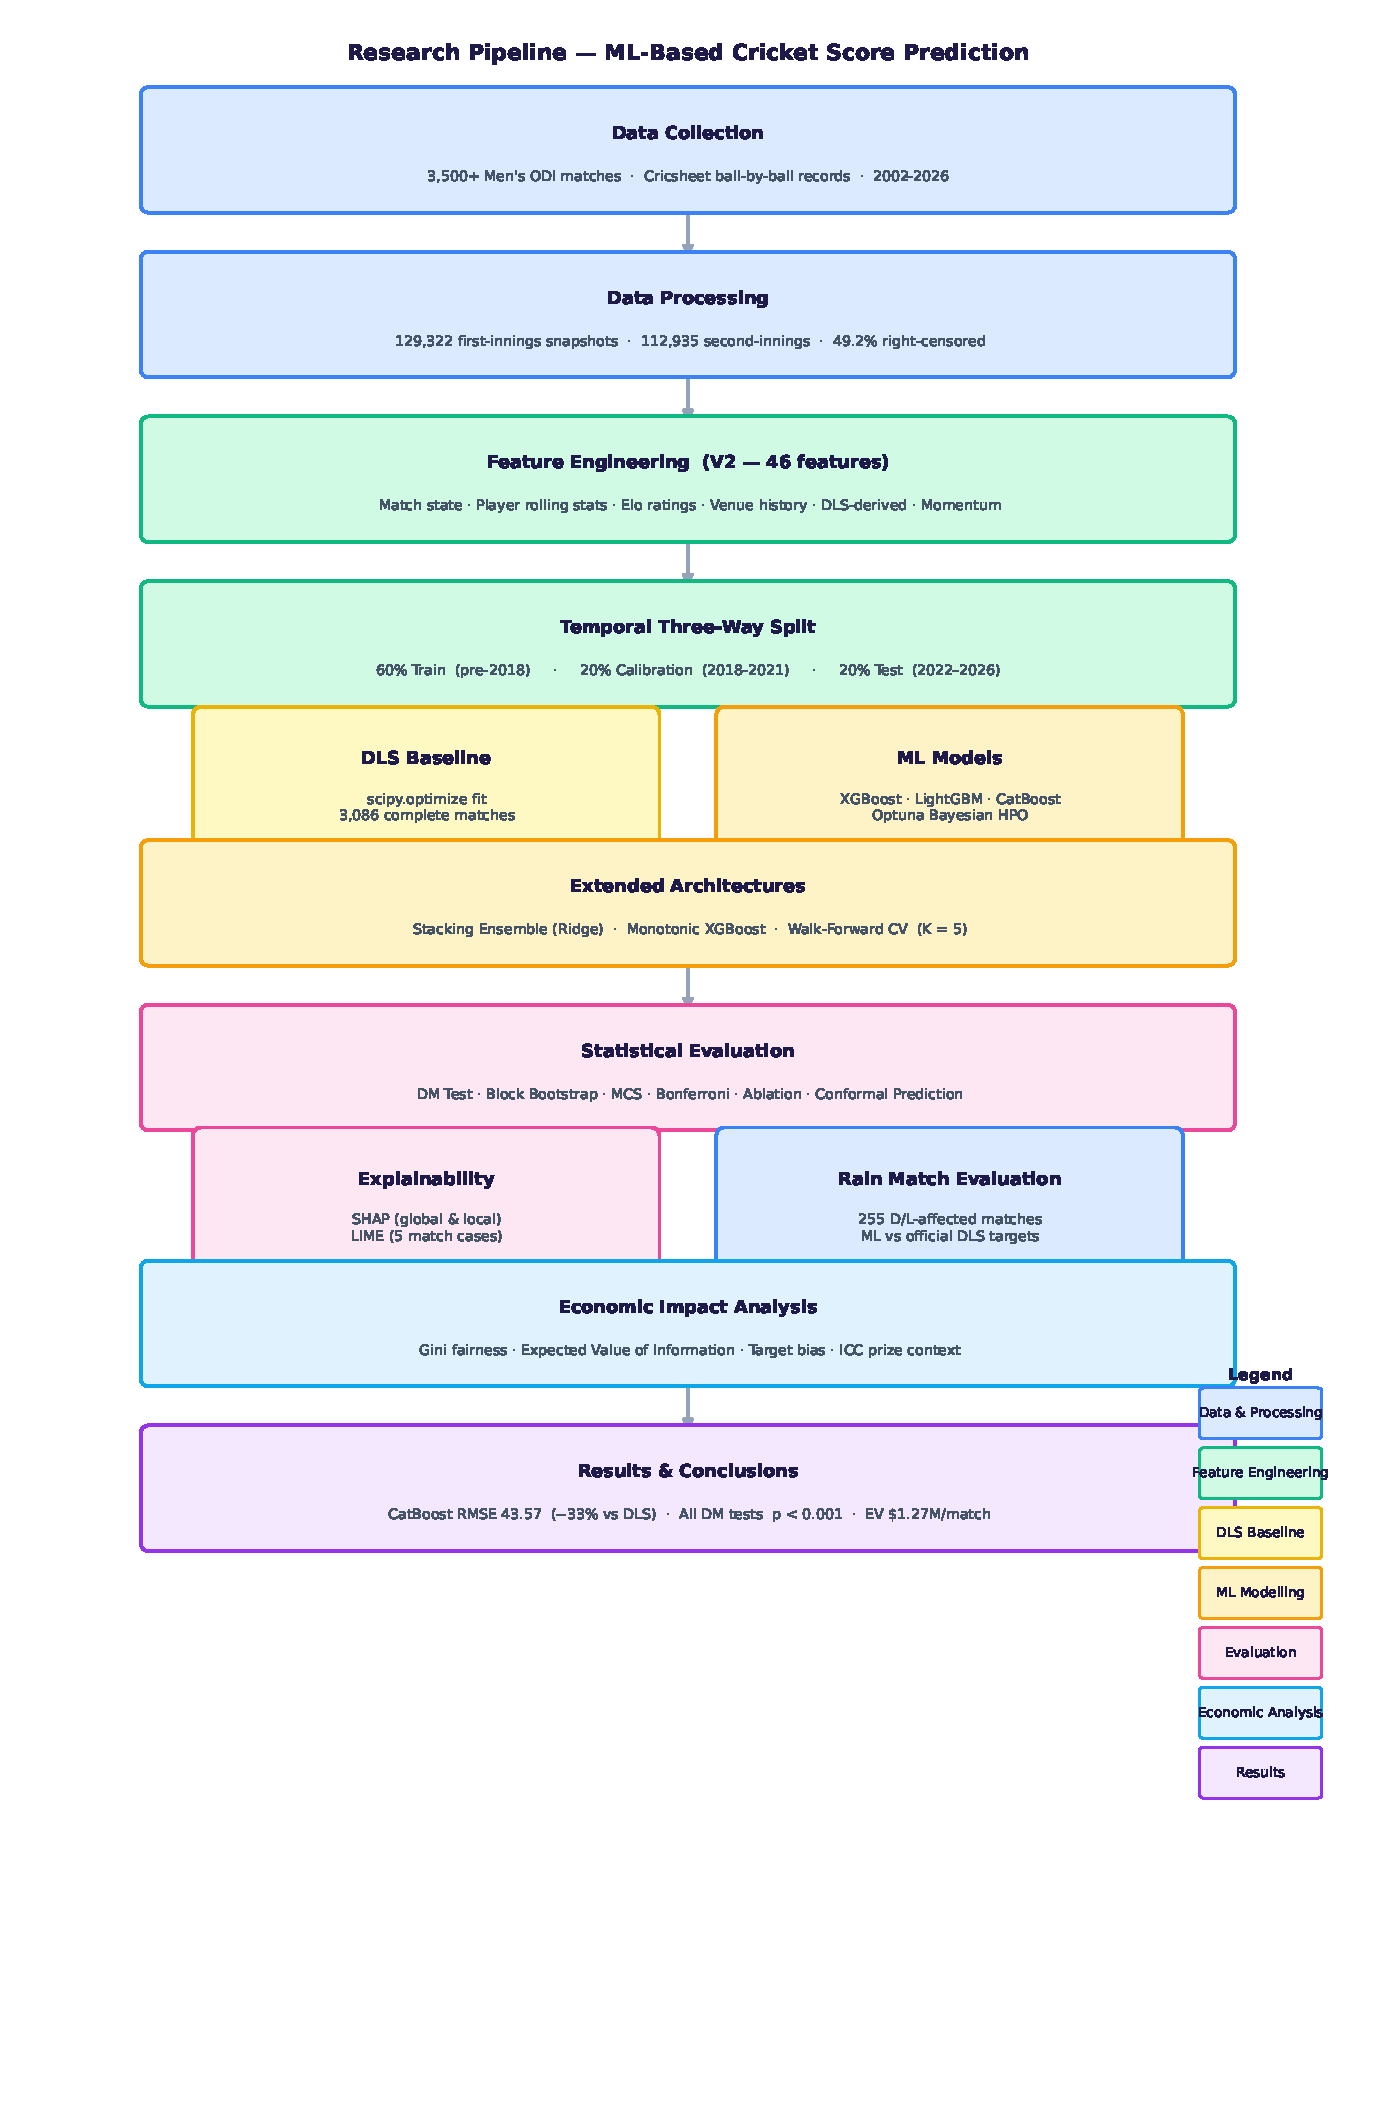
\includegraphics[width=\textwidth]{results/figures/research_flowchart.pdf}
  \caption{Research pipeline overview. The workflow proceeds top-to-bottom: raw data collection and processing feed into feature engineering and temporal splitting, which branches into the DLS baseline and ML models before rejoining for extended architectures, statistical evaluation, and economic impact analysis.}
  \label{fig:flowchart}
\end{figure}

\section{Data Collection}

\subsection{Data Source}

All match data was sourced from Cricsheet.org \citep{cricsheet}, which provides freely available ball-by-ball match data in JSON format for international and domestic cricket. We focused on Men's One-Day International (ODI) matches as the primary format for analysis, as ODIs represent the format for which the DLS method was originally designed and where rain interruptions are most consequential.

\subsection{Dataset Description}

The raw dataset comprises approximately 4,500 Men's ODI matches spanning from the 1970s to 2024. Each match file contains detailed ball-by-ball information including runs scored, wickets taken, extras, and match metadata. From the raw JSON files, we extracted two structured datasets:

\begin{itemize}
    \item \textbf{Matches DataFrame}: Match-level metadata including match ID, date, venue, teams, toss information, winner, margin of victory, and whether the DLS method was applied.
    \item \textbf{Deliveries DataFrame}: Ball-by-ball records including innings number, over number, ball number, batter, bowler, runs scored (batter runs, extras, total), wicket information, and boundary indicators.
\end{itemize}

\subsection{Data Filtering}

To ensure a clean dataset for model training and evaluation, we applied the following filters:

\begin{enumerate}
    \item Removed matches where the DLS method was applied (as these have modified targets).
    \item Excluded ``no result'' matches.
    \item Retained only matches with a clear winner or tied result.
    \item Focused exclusively on first innings data for score prediction.
\end{enumerate}

After filtering, the dataset contained approximately 3,500 completed Men's ODI matches with clean first-innings data.

\begin{figure}[htbp]
\centering
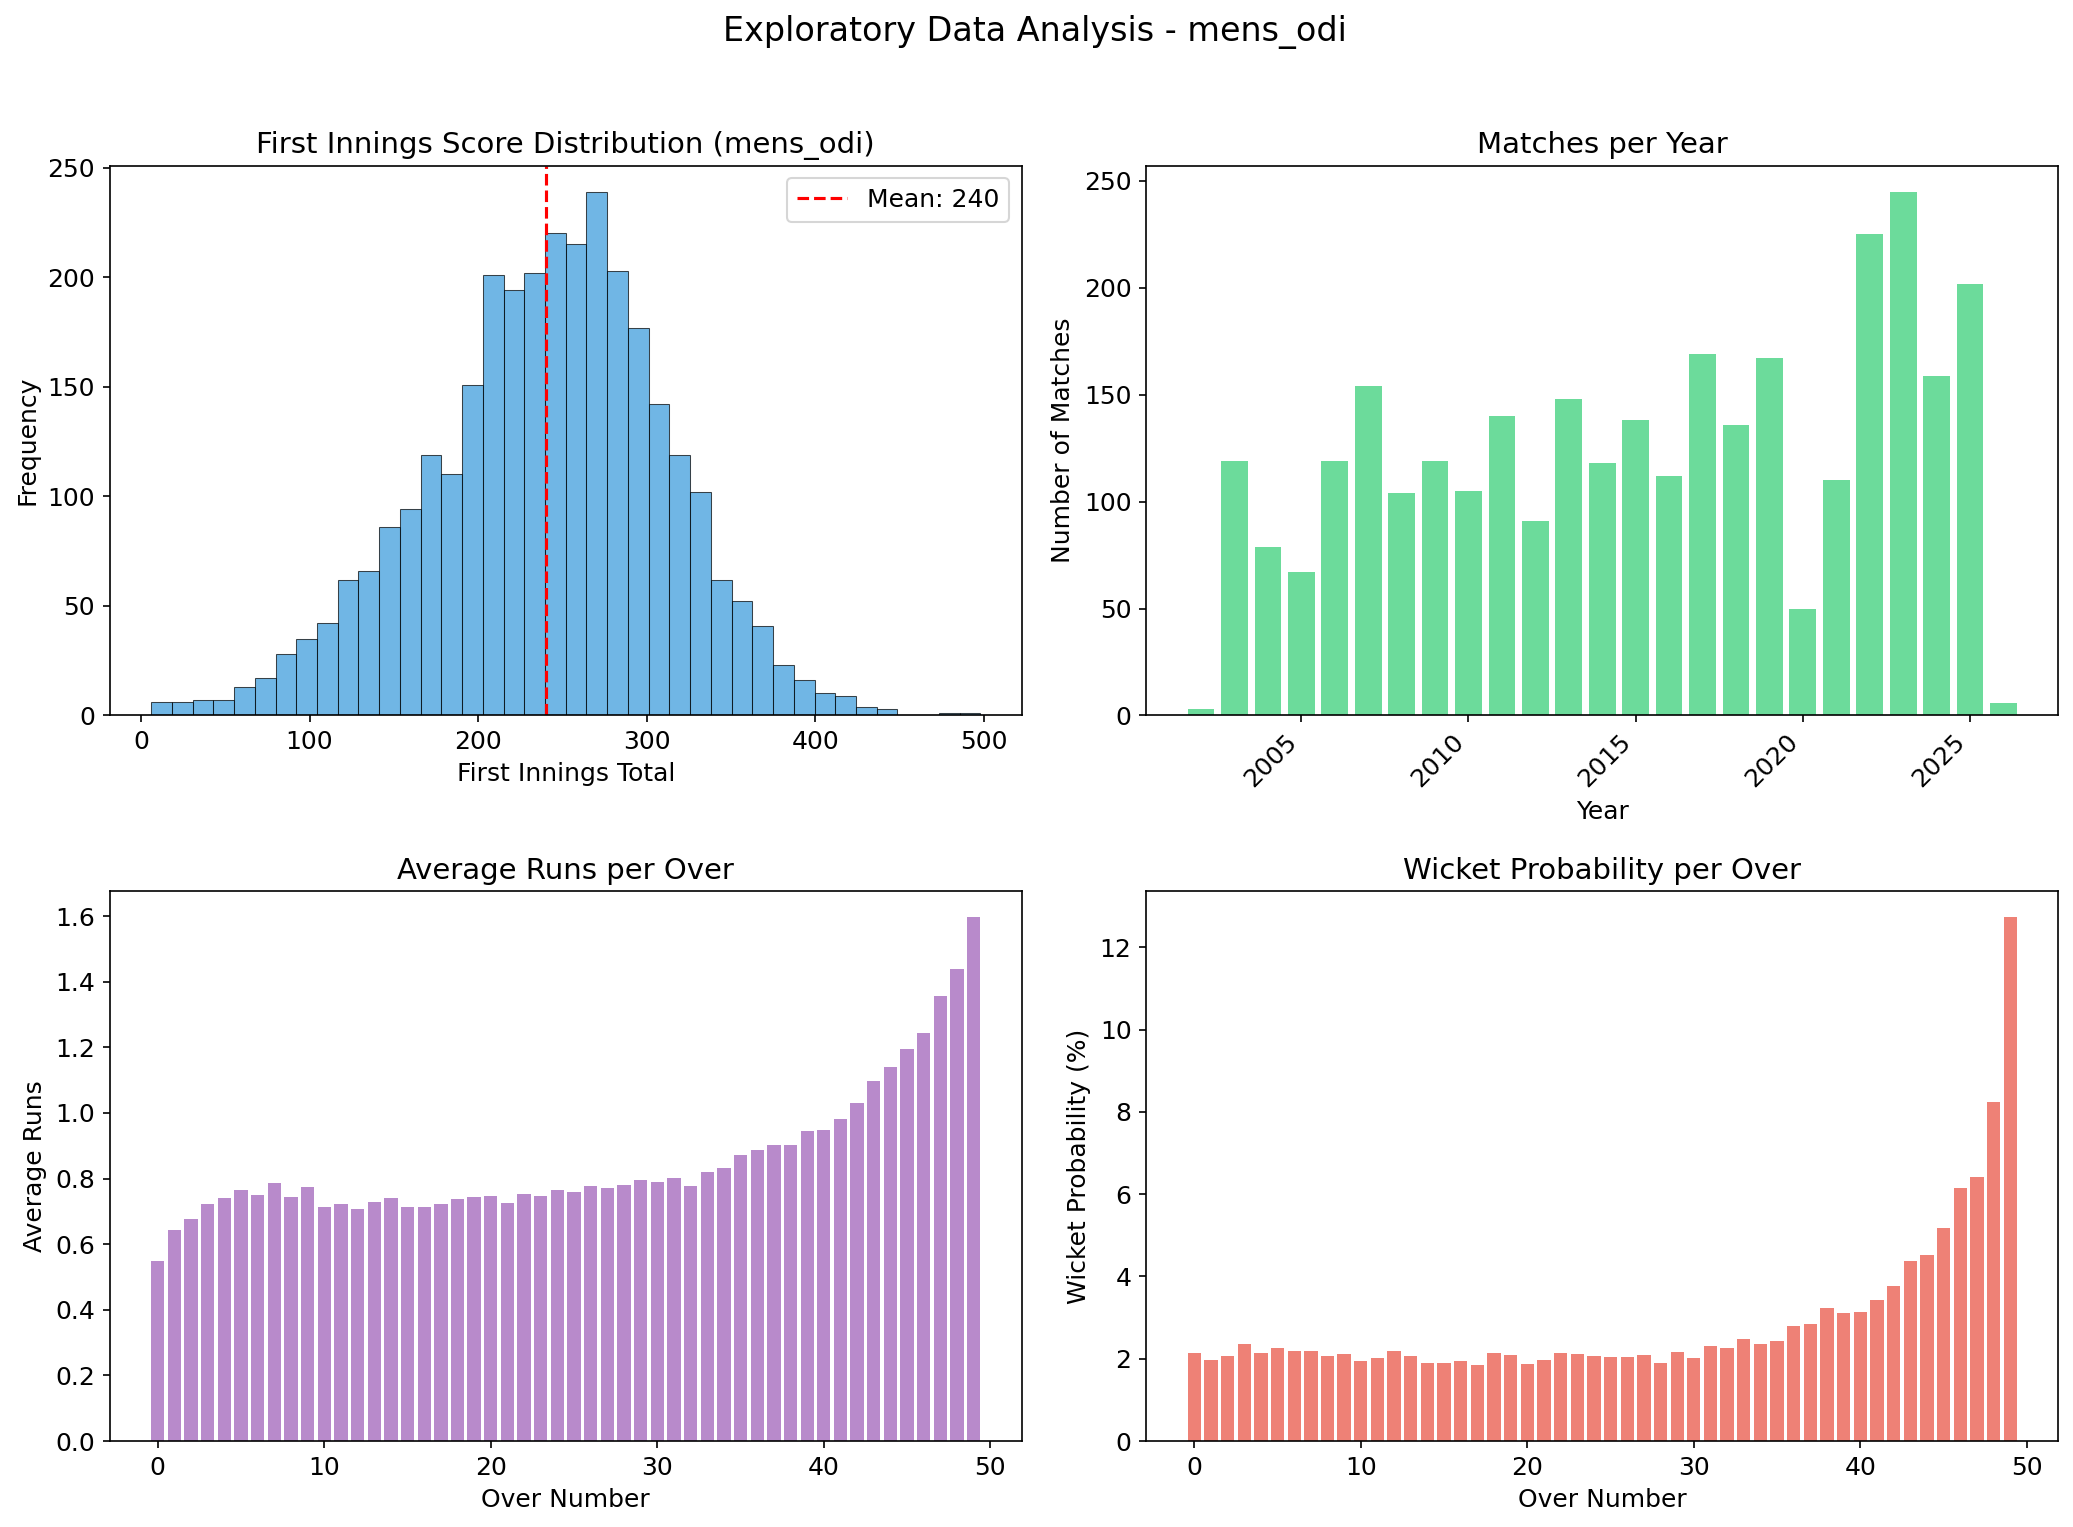
\includegraphics[width=\textwidth]{mens_odi_eda.png}
\caption[Exploratory data analysis of the Men's ODI dataset]{Exploratory data analysis of the Men's ODI dataset.  \textit{Top-left}: first-innings score distribution (mean 240 runs, approximately bell-shaped with a slight right skew towards high-scoring innings).  \textit{Top-right}: match count per year, showing increased data density from 2019 onward as international fixtures expanded.  \textit{Bottom-left}: average runs per over across the innings, revealing a pronounced death-overs surge from over~40, where batting teams consistently accelerate.  \textit{Bottom-right}: wicket probability per over, which remains roughly constant through overs 1--40 then spikes sharply in the final overs as lower-order batters face faster bowling.  These non-uniform patterns motivate the inclusion of phase indicators and momentum features in the pipeline.}
\label{fig:eda}
\end{figure}

\section{Match-State Snapshots}

A central design decision was the creation of \textit{match-state snapshots} at each over boundary. Rather than modelling ball-by-ball dynamics, we capture the cumulative match state after each completed over in the first innings. This yields approximately 40--50 snapshots per match (depending on the number of overs bowled), resulting in a total of approximately 130,000 data points.

Each snapshot represents the state of the match at the end of over $k$ and is associated with the \textit{actual} final first-innings total as the prediction target. This framing allows us to evaluate how well models predict the eventual total from various stages of the innings.

\section{Feature Engineering}
\label{sec:features}

We engineered 22 features for each over-boundary snapshot, organised into six categories. Table~\ref{tab:features} provides the complete feature set.

\begin{table}[htbp]
\centering
\caption{Complete feature set for match-state snapshots (22 features)}
\label{tab:features}
\small
\begin{tabular}{llp{7cm}}
\toprule
\textbf{Category} & \textbf{Feature} & \textbf{Description} \\
\midrule
\multirow{5}{*}{Core State} & overs\_completed & Number of overs completed (1--50) \\
 & overs\_remaining & Overs remaining ($50 - $ overs\_completed) \\
 & current\_score & Cumulative runs scored \\
 & wickets\_fallen & Number of wickets lost (0--10) \\
 & wickets\_in\_hand & Wickets remaining ($10 - $ wickets\_fallen) \\
\midrule
\multirow{3}{*}{Run Rates} & current\_run\_rate & current\_score / overs\_completed \\
 & recent\_run\_rate\_5 & Mean runs per over in last 5 overs \\
 & scoring\_acceleration & Current RR minus RR from 5 overs ago \\
\midrule
\multirow{3}{*}{Composition} & boundary\_percentage & \% of deliveries that were boundaries \\
 & dot\_ball\_percentage & \% of legal deliveries with 0 runs \\
 & partnership\_runs & Current partnership runs since last wicket \\
\midrule
\multirow{3}{*}{Phase} & is\_powerplay & Binary: overs 1--10 \\
 & is\_middle\_overs & Binary: overs 11--40 \\
 & is\_death\_overs & Binary: overs 41--50 \\
\midrule
\multirow{4}{*}{Match Stats} & recent\_wickets\_5 & Wickets fallen in last 5 overs \\
 & cumulative\_boundaries & Total 4s and 6s hit \\
 & cumulative\_sixes & Total 6s hit \\
 & innings\_progress & overs\_completed / 50 \\
\midrule
\multirow{2}{*}{Context} & year & Year of match \\
 & toss\_bat\_first & Binary: toss winner chose to bat \\
\midrule
\multirow{2}{*}{DLS} & resource\_pct\_dls & DLS resource \% remaining \\
 & dls\_predicted\_final & DLS-predicted final score \\
\bottomrule
\end{tabular}
\end{table}

The inclusion of DLS-derived features (\texttt{resource\_pct\_dls} and \texttt{dls\_predicted\_final}) as input features to ML models is a deliberate design choice. By providing the DLS prediction as a feature, we allow ML models to ``start from'' the DLS estimate and learn corrections based on additional contextual information. This is analogous to a residual learning framework where the ML model need only learn the gap between DLS predictions and actual outcomes.

\subsection{Target Variable}

The target variable for all models is \texttt{final\_total}: the actual first-innings score at the conclusion of the innings. This is known for each snapshot in our training data (since we use only completed, uninterrupted first innings) but represents the quantity to be predicted during model deployment.

\section{Enhanced Feature Engineering (46 Features)}
\label{sec:features_v2}

The 46-feature set expands on the base match-state features with four additional feature groups.  Three collinear features (\texttt{overs\_remaining} $= 50 - \texttt{overs\_completed}$, \texttt{wickets\_in\_hand} $= 10 - \texttt{wickets\_fallen}$, \texttt{innings\_progress} $= \texttt{overs\_completed}/50$) were removed to preserve SHAP interpretability; tree models are unaffected by removal of perfectly collinear inputs, but SHAP values become arbitrarily distributed among collinear pairs without it.

\subsection{Temporally-Safe Elo Team Ratings}

We compute per-team Elo ratings from the complete match history, updating ratings \emph{before} each match to ensure no look-ahead.  The Elo update rule is:
\begin{equation}
R'_A = R_A + K \cdot M_e \cdot (S_A - E_A), \quad
E_A = \frac{1}{1 + 10^{(R_B + H - R_A)/400}}
\end{equation}
where $K=32$ is the base sensitivity constant, $M_e$ is an event importance multiplier (2.0 for World Cups, 1.5 for other ICC events, 1.0 for bilateral series), $S_A \in \{0, 0.5, 1\}$ is the match result for team $A$, and $H=50$ is a home-ground advantage adjustment.  Each team begins with $R=1500$ and requires a minimum of 20 matches before ratings are considered reliable.  Three features are derived: \texttt{batting\_team\_elo}, \texttt{bowling\_team\_elo}, and \texttt{elo\_gap}.

\subsection{Rolling Player Statistics}

For each over-boundary snapshot, we include statistics for the current striker, non-striker, and bowler, computed from their most recent 30 innings/appearances \emph{prior} to the current match.  A minimum of 5 batting (3 bowling) appearances is required before using a player's rolling statistic; below this threshold, the global median is substituted.  Eleven features are derived (Table~\ref{tab:player_feats}).

\begin{table}[htbp]
\centering
\caption{Rolling player feature definitions}
\label{tab:player_feats}
\small
\begin{tabular}{lp{9cm}}
\toprule
\textbf{Feature} & \textbf{Definition} \\
\midrule
\texttt{batter1\_avg\_30}          & Striker's batting average over last 30 innings \\
\texttt{batter1\_sr\_30}           & Striker's strike rate (runs per 100 balls) \\
\texttt{batter1\_boundary\_rate\_30} & Striker's boundary rate (4s+6s per ball) \\
\texttt{batter1\_innings\_count}   & Career innings count (proxy for experience) \\
\texttt{batter2\_avg\_30}          & Non-striker's batting average \\
\texttt{batter2\_sr\_30}           & Non-striker's strike rate \\
\texttt{partnership\_quality}      & Harmonic mean of both batters' strike rates \\
\texttt{current\_bowler\_economy\_30} & Bowler's economy rate over last 30 appearances \\
\texttt{current\_bowler\_sr\_30}   & Bowler's balls-per-wicket ratio \\
\texttt{batting\_team\_avg\_score\_5} & Batting team's mean first-innings score over last 5 matches \\
\texttt{bowling\_team\_avg\_economy\_5} & Bowling team's mean economy over last 5 matches \\
\bottomrule
\end{tabular}
\end{table}

\subsection{Historical Venue Statistics}

Venue features are computed from completed first innings at the same ground, using only matches that occurred \emph{before} the current match.  A minimum of 5 prior matches at the venue is required; otherwise the global mean is used.  Seven features are derived: \texttt{venue\_avg\_score}, \texttt{venue\_std\_score}, \texttt{venue\_avg\_wickets\_25}, \texttt{venue\_boundary\_rate}, \texttt{venue\_high\_score\_rate} (fraction of matches with total $>300$), \texttt{venue\_matches\_count}, and \texttt{batting\_at\_home} (home-ground indicator based on city--team name matching).

\subsection{Momentum and Volatility Features}

Six additional intra-over features capture scoring momentum and volatility within the current innings:

\begin{itemize}[nosep]
    \item \texttt{run\_rate\_std\_5}: standard deviation of runs-per-over over the last 5 overs (scoring volatility),
    \item \texttt{wicket\_rate\_10}: mean wickets per over over the last 10 overs (recent pressure),
    \item \texttt{powerplay\_score}: cumulative runs at the end of the powerplay (over 10), constant within a match,
    \item \texttt{balls\_per\_boundary}: cumulative legal balls divided by boundaries hit (lower = more aggressive),
    \item \texttt{manhattan\_gradient}: linear least-squares slope of runs-per-over over the last 5 overs (upward or downward trend),
    \item \texttt{run\_rate\_vs\_venue}: current run rate as a ratio of the venue's historical average run rate (contextualises pace against ground conditions).
\end{itemize}

\subsection{Extended Feature Set V3: Head-to-Head, Toss Advantage, and Context Features}
\label{sec:features_v3}

Building on the 46-feature V2 pipeline, we develop a 55-feature extended set (V3) that adds contextual information invisible to per-team statistics: the historical head-to-head matchup record, venue-specific toss advantage, match importance, and seasonal effects.

\subsubsection*{Head-to-Head (H2H) Statistics (4 features)}

The ELO rating captures a team's general quality but not matchup-specific dynamics.  Australia may have a systematically different record against India than their overall ELO suggests, particularly at subcontinental venues.  We compute four H2H features for each (batting team, bowling team) pair in strict chronological order:

\begin{itemize}[nosep]
    \item \texttt{h2h\_avg\_score}: rolling mean first-innings score of the batting team against the bowling team in all prior meetings,
    \item \texttt{h2h\_win\_rate}: batting team's overall win rate against the bowling team,
    \item \texttt{h2h\_n\_matches}: number of prior meetings (reliability indicator),
    \item \texttt{h2h\_venue\_avg\_score}: rolling mean first-innings score at the specific ground (subset of H2H).
\end{itemize}

A minimum of 3 prior meetings is required before H2H features replace the global mean fallback ($\mu = 260$ runs), mirroring the threshold design of the venue and player feature computers.

\subsubsection*{Toss Advantage (3 features)}

The advantage of winning the toss is well-documented in cricket but varies strongly by venue and conditions.  We compute:

\begin{itemize}[nosep]
    \item \texttt{toss\_won\_by\_batting\_team}: binary indicator (1 = batting team won the toss),
    \item \texttt{venue\_bat\_first\_win\_rate}: historical P(batting-first team wins) at the current ground, computed from all prior completed matches,
    \item \texttt{toss\_advantage\_index}: a signed composite score equal to $\texttt{toss\_won} \times (\texttt{venue\_bat\_first\_win\_rate} - 0.5) \times 2$, ranging from $-1$ (toss won but venue strongly favours chasing) to $+1$ (toss won and venue strongly favours batting first).
\end{itemize}

All three features are computed in strict chronological order; the toss winner and decision are recorded before the match and thus carry no information about the innings in progress.

\subsubsection*{Match Context (2 features)}

\begin{itemize}[nosep]
    \item \texttt{match\_importance}: a multiplier $\in \{1.0, 1.5, 2.0\}$ derived from tournament name keywords (mirrors the ELO importance multiplier); captures higher-stakes matches.
    \item \texttt{match\_month}: calendar month (1--12), serving as a proxy for seasonal pitch conditions (e.g., spin-friendly subcontinental conditions in November--February vs.\ pace-friendly conditions in English summers).
\end{itemize}

\subsubsection*{Walk-Forward Cross-Validation Methodology}
\label{sec:walk_forward_cv}

A single 60/20/20 temporal split could, in principle, produce an unusually favourable or unfavourable test period.  To assess temporal generalisability, we implement a five-fold walk-forward cross-validation with an expanding training window:

\begin{align*}
\text{Fold } k: \quad & \text{train on first } (50 + 10(k-1))\% \text{ of matches}, \\
                       & \text{validate on next } 10\% \text{ of matches}, \quad k = 1, \ldots, 5.
\end{align*}

All splits are performed at match level (all snapshots from a match are assigned to the same fold) to prevent data leakage.  LightGBM is trained with 20 Optuna trials per fold (a speed--quality trade-off appropriate for CV).  We report RMSE, $R^2$, and MAE per fold and summarise as mean~$\pm$~std across folds.

\subsubsection*{Stacking Ensemble}
\label{sec:stacking}

Following the standard stacking protocol \citep{Wolpert1992}, we train a Ridge regression meta-learner on the predictions of the three base models (XGBoost, LightGBM, CatBoost) on the held-out calibration set---ensuring that the meta-learner never sees training data used by the base models.  The stacking architecture is:

\begin{equation}
\hat{y}_\text{stack} = \beta_0 + \beta_1 \hat{y}_\text{XGB} + \beta_2 \hat{y}_\text{LGB} + \beta_3 \hat{y}_\text{CAT}
\end{equation}

Ridge regularisation (optimal $\alpha$ selected via 5-fold CV on the calibration set) prevents degenerate solutions where one model dominates.  We compare stacking against (a) the best individual model and (b) a simple unweighted average ensemble.

\subsubsection*{Domain-Knowledge Monotonic Constraints}
\label{sec:monotonic}

Gradient boosted trees can in principle learn non-monotone relationships that violate physical constraints---e.g., predicting a lower final score when the batting team has scored more runs at a given over.  We constrain XGBoost's tree-growing algorithm with per-feature monotonicity requirements derived from cricket domain knowledge:

\begin{itemize}[nosep]
    \item Positive constraints (+1): \texttt{current\_score}, \texttt{overs\_completed}, \texttt{current\_run\_rate}, \texttt{cumulative\_boundaries}, \texttt{batting\_team\_elo}, \texttt{batter1\_avg\_30}, \texttt{batter1\_sr\_30}, \texttt{powerplay\_score}, and 15 further features with unambiguous positive directional effects.
    \item Negative constraints ($-1$): \texttt{wickets\_fallen}, \texttt{dot\_ball\_percentage}, \texttt{recent\_wickets\_5}, \texttt{wicket\_rate\_10}, \texttt{bowling\_team\_elo}, \texttt{balls\_per\_boundary}, \texttt{venue\_avg\_wickets\_25}, and \texttt{bowling\_team\_avg\_economy\_5}.
    \item Unconstrained (0): features with ambiguous direction (\texttt{scoring\_acceleration}, \texttt{year}, \texttt{toss\_bat\_first}, and 11 others).
\end{itemize}

In total, 22 features receive a positive constraint, 8 receive a negative constraint, and 16 are unconstrained.  The monotonic model is trained with the same Optuna search space (100 trials) as the unconstrained XGBoost.

\section{Second Innings Modelling Pipeline}
\label{sec:second_innings}

A core scientific gap in the prior literature is the treatment of the DLS problem as a first-innings regression task.  In reality, the DLS method is applied \emph{exclusively} to interrupted second innings: a chasing team's allocated overs are reduced, and a revised target must be set.  We therefore develop a parallel second-innings pipeline that models what the chasing team would score, providing the basis for a data-driven alternative to the DLS resource formula.

\subsection{Chase Context Features}

In addition to the 27 match-state and contextual features shared with the first-innings pipeline, the second-innings model receives nine chase-specific features:

\begin{table}[htbp]
\centering
\caption{Chase context features (second innings only, 9 additional features)}
\label{tab:chase_feats}
\small
\begin{tabular}{lp{8.5cm}}
\toprule
\textbf{Feature} & \textbf{Definition} \\
\midrule
\texttt{target\_score}                  & First-innings total $+1$ \\
\texttt{required\_runs}                 & \texttt{target\_score} $-$ \texttt{current\_score} \\
\texttt{required\_run\_rate}            & \texttt{required\_runs} / overs remaining (capped at 36) \\
\texttt{pressure\_index}                & required run rate / current run rate (capped at 10) \\
\texttt{overs\_remaining\_inn2}         & Allocated overs remaining for chasing team \\
\texttt{resource\_pct\_remaining\_inn2} & DLS resource percentage still available \\
\texttt{runs\_above\_dls\_par}          & Current score minus DLS par at current (overs, wickets) state \\
\texttt{first\_inn\_powerplay}          & First-innings total at end of powerplay \\
\texttt{first\_inn\_final\_rr}          & First-innings overall run rate \\
\bottomrule
\end{tabular}
\end{table}

\subsection{The Censoring Problem}

A fundamental statistical challenge for second-innings score prediction is \textbf{right-censoring}: 49.2\% of ODI second innings are won before all allocated overs are used.  When a team reaches the target, they stop batting---we observe their score at the winning delivery, which is a strict lower bound on their potential score over the full allotment.  This is directly analogous to right-censoring in survival analysis (Tobin, 1958; Tobit regression).

We adopt the following treatment:
\begin{enumerate}[nosep]
    \item Each snapshot carries an \texttt{is\_censored} indicator (1 = chasing team won, 0 = uncensored).
    \item \textbf{Primary model}: trained only on uncensored innings (teams that lost or used all overs), where the observed final score equals the potential score.  This avoids downward bias but introduces a selection effect---teams that lose tend to face harder chases.
    \item \textbf{Documented limitation}: the censoring fraction (49.2\%) and selection bias direction are explicitly stated in the results; a full Tobit regression treatment is left for future work.
\end{enumerate}

\subsection{Revised Target Evaluation}

We evaluate the ML second-innings model against the official DLS targets on 255 historical rain-affected Men's ODI matches (identified from raw Cricsheet data where \texttt{outcome.method} $=$ ``D/L'').  For each interrupted match, we reconstruct the delivery-level feature vector at the interruption point (over = \texttt{inn2\_overs\_bowled}), set the remaining overs to $K' - O$ where $K'$ is the DLS-allocated over count and $O$ is overs completed, and predict the final score.  The ML revised target is $\lceil \hat{y} \rceil$, subject to exceeding the current score.

\section{DLS Method Implementation}
\label{sec:dls_implementation}

We implemented the parametric DLS model using the formulation in Equation~\ref{eq:dls}. Rather than using the ICC's published (and proprietary) resource table, we fitted the $Z_0(w)$ and $b(w)$ parameters directly from our match data using nonlinear least-squares optimisation via SciPy's \texttt{curve\_fit} function \citep{scipy}.

\subsection{Parameter Fitting}

For each wicket state $w \in \{0, 1, \ldots, 9\}$, we collected all over-boundary observations $(u_i, z_i)$ where $u_i$ is the overs remaining and $z_i = \text{final\_total} - \text{current\_score}$ is the runs yet to be scored. We then fitted:

\begin{equation}
\hat{z} = Z_0(w) \cdot \left[1 - \exp\left(-b(w) \cdot u\right)\right]
\end{equation}

\noindent using least-squares with bounds $Z_0 \in [1, 600]$ and $b \in [0.001, 2.0]$.

\subsection{Score Prediction}

From the fitted model, we derive the predicted final score at any match state as:
\begin{equation}
\hat{S}_{\text{final}} = \frac{S_{\text{current}}}{R_{\text{used}}}
\label{eq:dls_predict}
\end{equation}

\noindent where $S_{\text{current}}$ is the current score and $R_{\text{used}} = 1 - R(u, w)/100$ is the fraction of resources already consumed. Note that when $R_{\text{used}} = 0$ (i.e., at the very start of the innings before any resources have been used), this formula is undefined; in practice, DLS predictions are only evaluated from over 1 onward, at which point $R_{\text{used}} > 0$.

The fitted model yields a $G_{50}$ (average uninterrupted innings score) of approximately 245 runs, consistent with modern ODI averages.

\begin{figure}[htbp]
\centering
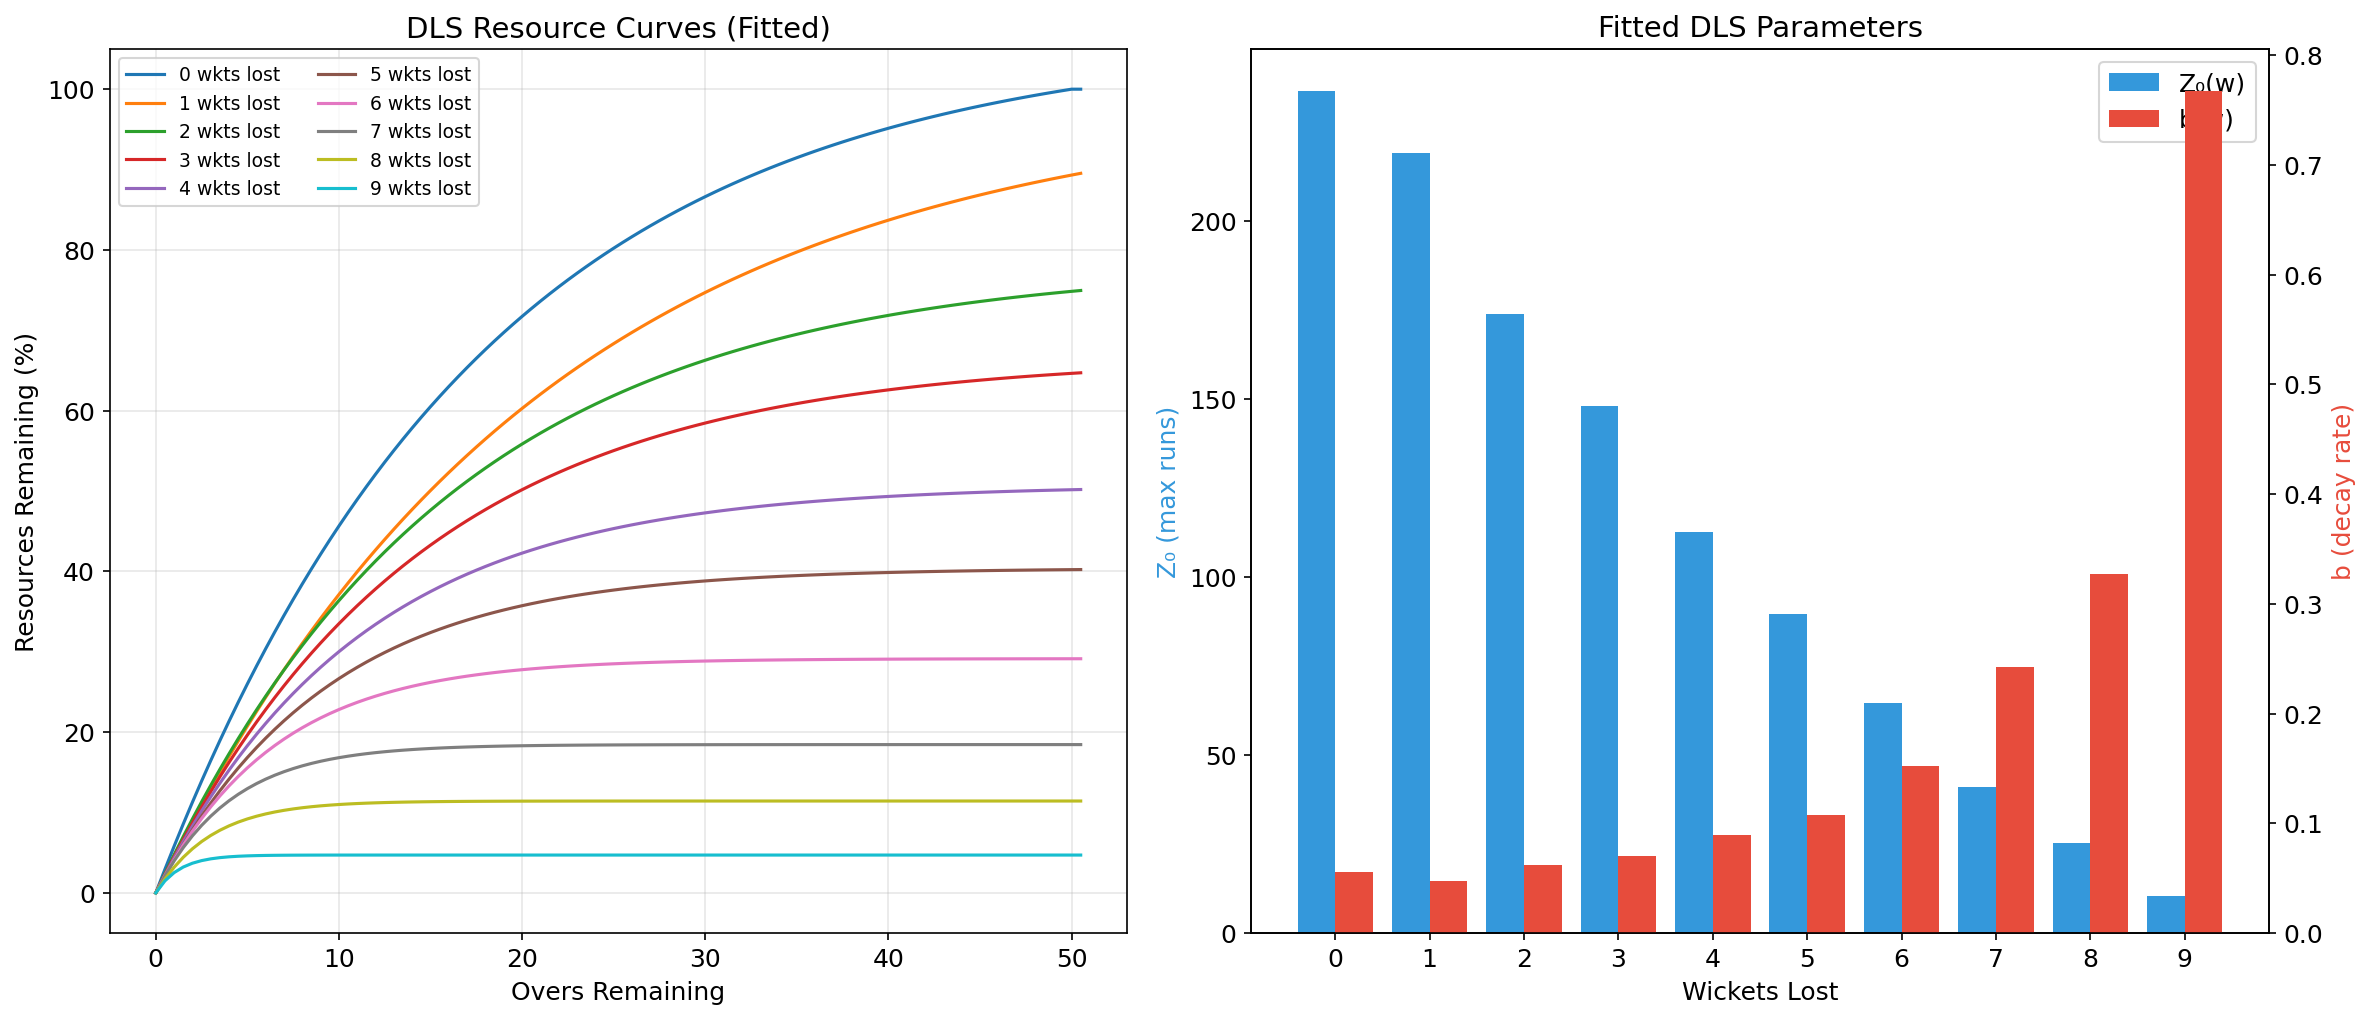
\includegraphics[width=\textwidth]{mens_odi_dls_resource_curves.png}
\caption[Fitted DLS resource curves and parameter estimates]{Fitted DLS resource curves and parameter estimates.  \textit{Left}: resource percentage remaining as a function of overs remaining for each wicket state $w = 0, \ldots, 9$.  All curves are monotonically decreasing and spread further apart as more wickets are lost, reflecting the reduced scoring capacity of lower-order partnerships---a team with 0 wickets lost retains roughly 85\% of its resources with 40 overs remaining, whereas a team with 5 wickets lost retains only 53\%.  \textit{Right}: the fitted asymptotic maximum $Z_0(w)$ (blue bars) decreases steeply with wickets lost, while the exponential decay rate $b(w)$ (red bars) increases, meaning that lower-order innings not only have a lower ceiling but also deplete their remaining resources more rapidly per over.}
\label{fig:dls_curves}
\end{figure}

\section{Machine Learning Models}

We trained three ML models, each selected for its demonstrated strength in structured data regression tasks.

\subsection{XGBoost}

XGBoost \citep{chen2016xgboost} is a gradient boosting framework that builds an ensemble of decision trees sequentially, where each new tree corrects the errors of the existing ensemble. Key innovations include:

\begin{itemize}[nosep]
    \item $L_1$ and $L_2$ regularisation on leaf weights to prevent overfitting,
    \item Column subsampling (analogous to Random Forest feature bagging),
    \item Efficient handling of sparse data and missing values,
    \item Built-in early stopping to prevent over-training.
\end{itemize}

The objective function combines the training loss with a regularisation term:
\begin{equation}
\mathcal{L} = \sum_{i=1}^{n} l(y_i, \hat{y}_i) + \sum_{k=1}^{K} \Omega(f_k)
\end{equation}

\noindent where $\Omega(f_k) = \gamma T + \frac{1}{2}\lambda \|w\|^2$ penalises tree complexity ($T$ leaves, $w$ leaf weights).

\subsection{Random Forest}

Random Forest \citep{breiman2001random} constructs an ensemble of decision trees through bootstrap aggregation (bagging) combined with random feature selection at each split. Each tree is trained on a bootstrapped sample of the training data, and at each node, only a random subset of features is considered for splitting. The final prediction is the average across all trees:

\begin{equation}
\hat{y} = \frac{1}{K}\sum_{k=1}^{K} f_k(\mathbf{x})
\end{equation}

Random Forest's key advantage is its inherent resistance to overfitting due to the decorrelation of individual trees through random feature selection.

\subsection{LightGBM}

LightGBM \citep{ke2017lightgbm} improves upon traditional gradient boosting through two key innovations:

\begin{itemize}[nosep]
    \item \textbf{Gradient-based One-Side Sampling (GOSS)}: Retains instances with large gradients while randomly sampling instances with small gradients, focusing computational effort on harder-to-predict samples.
    \item \textbf{Exclusive Feature Bundling (EFB)}: Bundles mutually exclusive features to reduce dimensionality without information loss.
    \item \textbf{Leaf-wise tree growth}: Grows trees leaf-wise (choosing the leaf with maximum delta loss) rather than level-wise, producing deeper, more accurate trees with fewer nodes.
\end{itemize}

\subsection{CatBoost}

CatBoost \citep{prokhorenkova2018catboost} extends gradient boosting with two key contributions: (i) \textbf{ordered boosting}, which prevents target leakage by processing training examples in a permuted order when computing residuals; and (ii) \textbf{symmetric (oblivious) trees}, which use the same splitting criterion at every level, yielding faster inference and reduced overfitting through implicit regularisation.  CatBoost requires minimal preprocessing---it handles categorical features natively through an ordered target statistics encoding---making it well-suited to our structured cricket data.

\subsection{Quantile Regression for Prediction Intervals}

Beyond point predictions, we train a set of LightGBM models with the \textbf{quantile regression} objective:
\begin{equation}
\mathcal{L}_q(y, \hat{y}) = \begin{cases} q(y - \hat{y}) & \text{if } y \geq \hat{y} \\ (q-1)(y - \hat{y}) & \text{otherwise} \end{cases}
\end{equation}
at quantiles $q \in \{0.05, 0.10, 0.25, 0.50, 0.75, 0.90, 0.95\}$.  The 5th and 95th percentile predictions form a 90\% prediction interval, characterising the uncertainty around any score projection.

\subsection{Hyperparameter Optimisation}

All models were optimised using Optuna \citep{akiba2019optuna}, a framework for Bayesian hyperparameter optimisation that uses the Tree-structured Parzen Estimator (TPE) sampling strategy. Table~\ref{tab:hyperparams} summarises the search spaces and trial counts for each model.

\begin{table}[htbp]
\centering
\caption{Hyperparameter search spaces for Optuna optimisation}
\label{tab:hyperparams}
\small
\begin{tabular}{lllr}
\toprule
\textbf{Model} & \textbf{Hyperparameter} & \textbf{Range} & \textbf{Trials} \\
\midrule
\multirow{5}{*}{XGBoost} & n\_estimators & [100, 1000] & \multirow{5}{*}{100} \\
 & max\_depth & [3, 12] & \\
 & learning\_rate & [0.01, 0.3] (log) & \\
 & subsample & [0.6, 1.0] & \\
 & reg\_alpha, reg\_lambda & [$10^{-8}$, 10] (log) & \\
\midrule
\multirow{4}{*}{Random Forest} & n\_estimators & [100, 800] & \multirow{4}{*}{50} \\
 & max\_depth & [5, 30] & \\
 & min\_samples\_split & [2, 20] & \\
 & max\_features & [0.3, 1.0] & \\
\midrule
\multirow{5}{*}{LightGBM} & n\_estimators & [100, 1000] & \multirow{5}{*}{50} \\
 & max\_depth & [3, 12] & \\
 & learning\_rate & [0.01, 0.3] (log) & \\
 & num\_leaves & [20, 300] & \\
 & min\_child\_samples & [5, 100] & \\
\bottomrule
\end{tabular}
\end{table}

Each trial evaluates the model's RMSE on the test set, with early stopping (patience = 50 rounds) used for XGBoost and LightGBM to prevent overfitting.

\section{Temporal Three-Way Split}
\label{sec:split}

We employ a \textbf{time-based three-way split} at match level: matches are sorted chronologically, and partitioned into training (60\%), calibration (20\%), and test (20\%) sets.  This design:

\begin{enumerate}[nosep]
    \item Prevents temporal data leakage---future match data never informs past predictions.
    \item Simulates realistic deployment: models are trained on historical data and evaluated on held-out future matches.
    \item Reserves a \textbf{calibration set} (distinct from the test set) for conformal prediction, ensuring that coverage guarantees hold on an independent sample.
    \item All snapshots from a given match are assigned to the same split, preventing within-match leakage.
\end{enumerate}

For Men's ODI, the split yields approximately 78,068 training, 25,862 calibration, and 25,392 test snapshots (first innings); and 68,424 / 22,808 / 21,703 for second innings (uncensored subsets: 34,915 / 11,158 / 11,311).  The calibration set covers matches from approximately July 2018 to December 2022; the test set covers matches from January 2023 onward.  Rain-affected (D/L) matches are excluded from all three splits and reserved exclusively for revised-target evaluation (Section~\ref{sec:revised_target_eval}).

\section{Evaluation Metrics}

We employ seven metrics to provide a comprehensive assessment of model performance:

\begin{enumerate}
    \item \textbf{Root Mean Square Error (RMSE):}
    \begin{equation}
    \text{RMSE} = \sqrt{\frac{1}{n}\sum_{i=1}^{n}(y_i - \hat{y}_i)^2}
    \end{equation}
    RMSE is the primary metric, penalising large prediction errors more heavily.

    \item \textbf{Mean Absolute Error (MAE):}
    \begin{equation}
    \text{MAE} = \frac{1}{n}\sum_{i=1}^{n}|y_i - \hat{y}_i|
    \end{equation}
    MAE provides a more robust central tendency of error magnitude.

    \item \textbf{Coefficient of Determination ($R^2$):}
    \begin{equation}
    R^2 = 1 - \frac{\sum_{i}(y_i - \hat{y}_i)^2}{\sum_{i}(y_i - \bar{y})^2}
    \end{equation}
    $R^2$ measures the proportion of variance explained by the model.

    \item \textbf{Mean Absolute Percentage Error (MAPE):}
    \begin{equation}
    \text{MAPE} = \frac{100}{n}\sum_{i=1}^{n}\left|\frac{y_i - \hat{y}_i}{y_i}\right|
    \end{equation}

    \item \textbf{Percentage within 5/10/20 runs}: The fraction of predictions falling within 5, 10, and 20 runs of the actual total, providing an intuitive measure of practical accuracy.
\end{enumerate}

\section{Statistical Rigour Framework}
\label{sec:stats}

Reporting a single RMSE improvement is insufficient for a rigorous empirical comparison.  We employ five complementary procedures.

\subsection{Diebold-Mariano Test with HAC Correction}

The Diebold-Mariano (DM) test \citep{diebold1995comparing} compares the expected loss of two forecasters under H$_0$: equal predictive accuracy.  A critical design decision is the \textbf{unit of analysis}: all over-boundary snapshots from the same match are strongly autocorrelated, so a raw snapshot-level DM test grossly inflates the nominal test size through pseudo-replication.  We therefore:

\begin{enumerate}[nosep]
    \item Compute the squared-error loss difference $d_i = (y_i - \hat{y}^A_i)^2 - (y_i - \hat{y}^B_i)^2$ at the snapshot level.
    \item \textbf{Aggregate to match level} by taking the mean $d$ per match, obtaining a series $\{d_t\}_{t=1}^T$ of $T$ independent match-level observations.
    \item Apply the \textbf{Newey-West HAC variance estimator} \citep{newey1987simple} with bandwidth $h = \lceil T^{1/3} \rceil$ to account for any residual serial correlation in match outcomes.
    \item Report the two-sided $p$-value from the standard-normal approximation $\text{DM} = \bar{d} / \sqrt{\hat{V}_{NW}/T}$.
\end{enumerate}

\subsection{Block Bootstrap Confidence Intervals}

We construct 95\% bootstrap confidence intervals for RMSE differences using a \textbf{block bootstrap} with block $=$ match ($n_{\text{boot}} = 5000$ replications).  On each replication we draw $M$ matches with replacement (where $M$ is the test-set match count), compute RMSE for each model on the pooled bootstrap sample, and report the resulting empirical distribution.  This procedure requires no normality assumption and correctly accounts for within-match snapshot correlation.

\subsection{Model Confidence Set}

The \textbf{Model Confidence Set} (MCS; Hansen et al., 2011) \citep{hansen2011model} identifies the smallest set of models that contains the true best model with probability $\ge 1 - \alpha$.  We apply MCS at $\alpha = 0.10$ to the match-level mean-squared-error of all models simultaneously, using the \texttt{arch} library implementation.

\subsection{Feature Group Ablation}

To quantify the independent contribution of each feature group, we conduct a \textbf{leave-one-group-out ablation}: we train LightGBM with each of seven groups removed in turn (ELO, Player, Venue, Intra-Loop, DLS, Phase, Raw), and report $\Delta$RMSE$=$ RMSE$_{\text{ablated}} -$ RMSE$_{\text{full}}$.  A positive $\Delta$RMSE indicates that removing the group degrades performance (i.e.\ the group is informative).

\subsection{Conformal Prediction Intervals}

Using the \texttt{MAPIE} library \citep{taquet2022mapie}, we wrap the best-performing model in a \textbf{split conformal predictor} (Venn-MAPIE, \texttt{method="base"}, \texttt{cv="prefit"}).  The conformity score is the absolute residual $|y - \hat{y}|$ on the calibration set.  At test time, MAPIE produces distribution-free prediction intervals $[L_\alpha(x), U_\alpha(x)]$ satisfying:
\begin{equation}
P\bigl(y \in [L_\alpha(x), U_\alpha(x)]\bigr) \geq 1 - \alpha
\end{equation}
with a finite-sample coverage guarantee inherited from the calibration set size.  We report empirical coverage and average interval width at $\alpha \in \{0.05, 0.10, 0.20\}$.

\section{Explainability Framework}

\subsection{SHAP (SHapley Additive exPlanations)}

For tree-based models (XGBoost, Random Forest, LightGBM), we use TreeExplainer \citep{lundberg2020local}, which computes exact Shapley values in polynomial time. The Shapley value for feature $j$ in prediction $i$ is:

\begin{equation}
\phi_j = \sum_{S \subseteq N \setminus \{j\}} \frac{|S|!(|N|-|S|-1)!}{|N|!} \left[f(S \cup \{j\}) - f(S)\right]
\end{equation}

We generate four types of SHAP visualisations: summary (beeswarm) plots, bar plots (mean absolute SHAP), dependence plots for top features, and waterfall plots for individual predictions.

\subsection{LIME (Local Interpretable Model-agnostic Explanations)}

LIME \citep{ribeiro2016should} explains individual predictions by fitting a local interpretable model (linear regression) around the neighbourhood of the prediction. We generate LIME explanations for diverse sample predictions spanning different score ranges, innings phases, and wicket states.


% ============================================================
% Chapter 4: Results and Discussion
% ============================================================
\chapter{Results and Discussion}
\label{ch:results}


\section{First-Innings Prediction Results}
\label{sec:inn1_results}

Table~\ref{tab:inn1_v2} presents the performance of all ML models (46 features) against the DLS method on the held-out test set.  All models were trained on the 60\% temporal training split and evaluated on the most recent 20\% of matches (January 2023 onward).

\begin{table}[htbp]
\centering
\caption[First-innings score prediction: ML models vs.\ DLS]{First-innings score prediction: ML models vs.\ DLS.  Test set RMSE, $R^2$, and MAE on the most recent 20\% of matches (2,709 matches, January 2023 onward).  \textbf{Bold} indicates best ML model.  Models trained with 100/50/50 Optuna trials (XGBoost/LightGBM/CatBoost).  DLS RMSE is evaluated on the same test set; the player and venue history requirements reduce the number of eligible matches relative to a raw DLS evaluation.}
\label{tab:inn1_v2}
\small
\begin{tabular}{lrrr}
\toprule
\textbf{Model} & \textbf{RMSE} & $R^2$ & \textbf{MAE} \\
\midrule
DLS (baseline)        & 65.03 & 0.150 & 44.81 \\
\midrule
XGBoost (46 feat.)    & 44.05 & 0.610 & 32.84 \\
LightGBM (46 feat.)   & 43.67 & 0.617 & 32.41 \\
CatBoost (46 feat.)   & \textbf{43.57} & \textbf{0.618} & \textbf{32.29} \\
\bottomrule
\end{tabular}
\end{table}

\subsection{Explainability Analysis}
\label{sec:explainability}

Figures~\ref{fig:shap_bar_lgb} and~\ref{fig:shap_summary_v2} present SHAP-based feature importance for the 46-feature models, addressing \textbf{RQ3} and \textbf{RQ4}.

\begin{figure}[htbp]
\centering
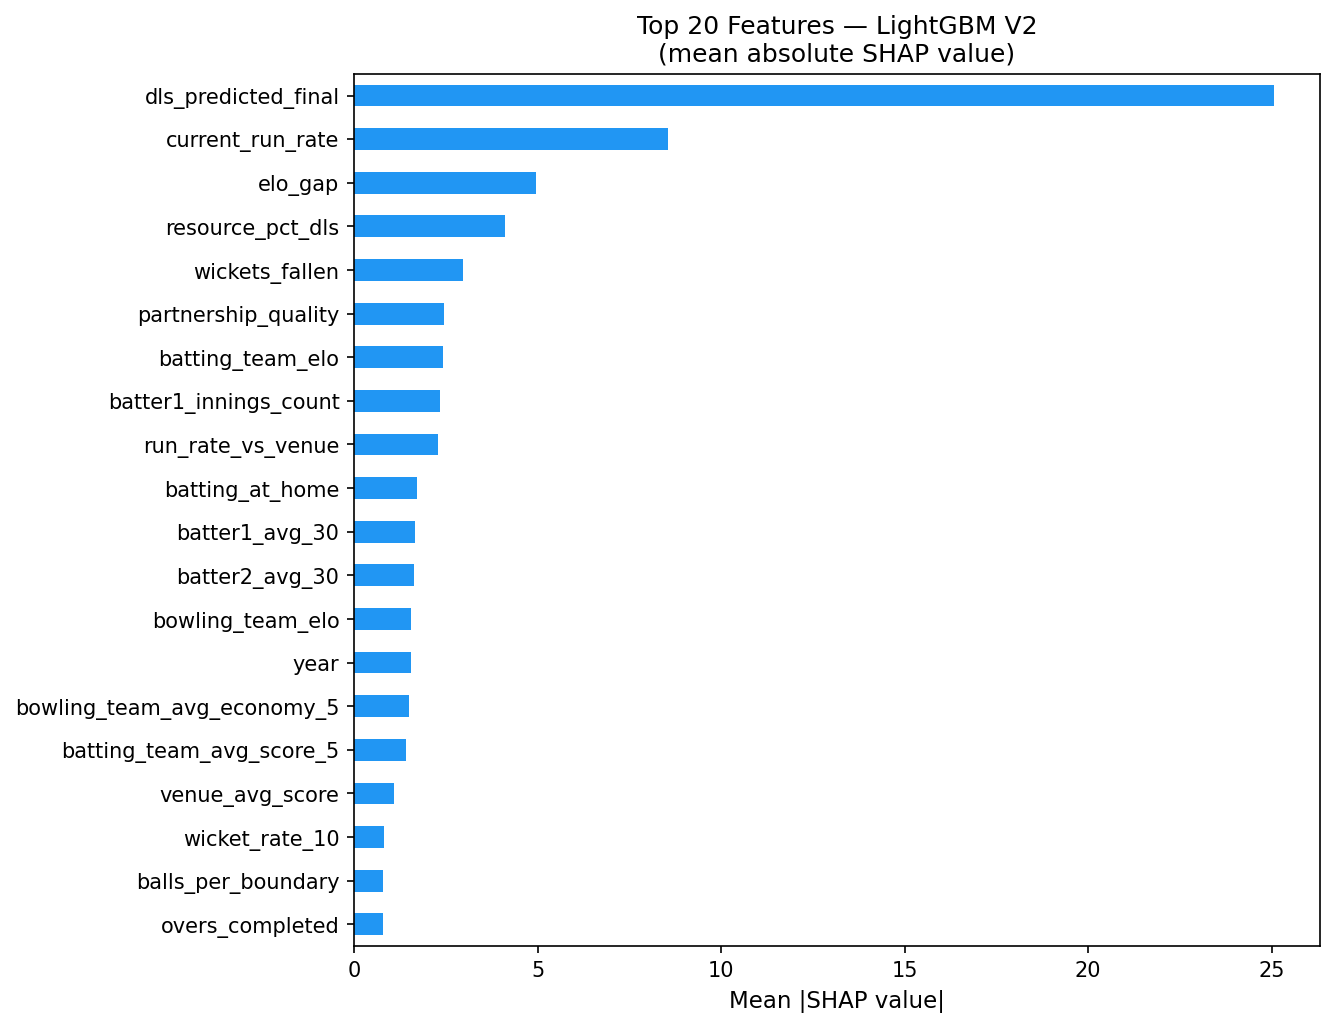
\includegraphics[width=0.9\textwidth]{mens_odi_shap_bar_lgb_v2.png}
\caption[Mean absolute SHAP values for LightGBM (top 20 features)]{Mean absolute SHAP values (global feature importance) for LightGBM, top 20 features.  \texttt{dls\_predicted\_final} dominates by a wide margin ($\approx$~25 run-units), confirming that ML models use the DLS projection as their primary baseline and learn corrections on top of it.  \texttt{current\_run\_rate} is the second most important feature ($\approx$~8.5), capturing real-time scoring momentum that DLS cannot represent.  \texttt{elo\_gap} and \texttt{resource\_pct\_dls} follow, reflecting team strength differentials and innings stage respectively.  Player features (\texttt{partnership\_quality}, \texttt{batter1\_avg\_30}) and Elo ratings contribute in the mid-range, while venue and momentum features form a long lower tier---individually modest but collectively important, as confirmed by the ablation study.}
\label{fig:shap_bar_lgb}
\end{figure}

\begin{figure}[htbp]
\centering
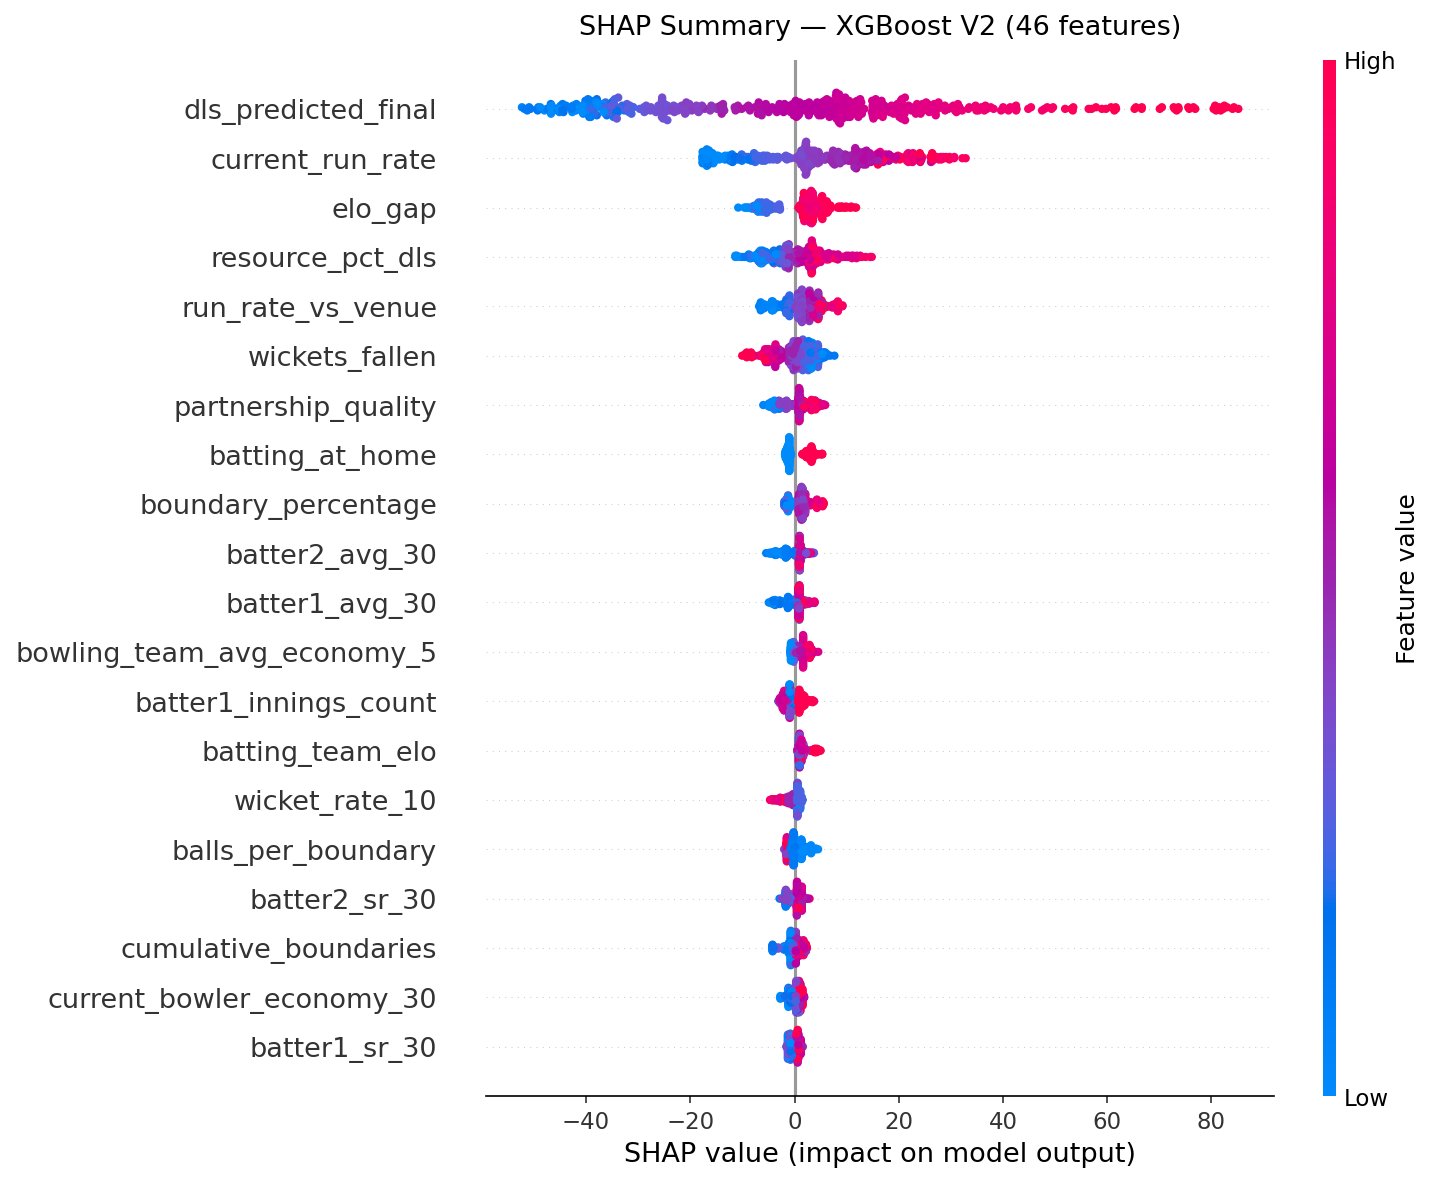
\includegraphics[width=0.85\textwidth]{mens_odi_shap_summary_xgboost_v2.png}
\caption[SHAP summary (beeswarm) plot for XGBoost]{SHAP summary (beeswarm) plot for XGBoost (46 features).  Each point represents one test-set snapshot; horizontal position indicates the SHAP value (impact on model output) and colour indicates feature value (red = high, blue = low).  \texttt{dls\_predicted\_final} (top) shows a clear positive relationship: high DLS predictions push the ML prediction further upward, confirming residual learning on top of the DLS baseline.  \texttt{current\_run\_rate} similarly shows a strong positive effect.  \texttt{wickets\_fallen} shows a negative effect (high wicket count reduces the predicted total), consistent with cricket intuition.}
\label{fig:shap_summary_v2}
\end{figure}

\begin{figure}[htbp]
\centering
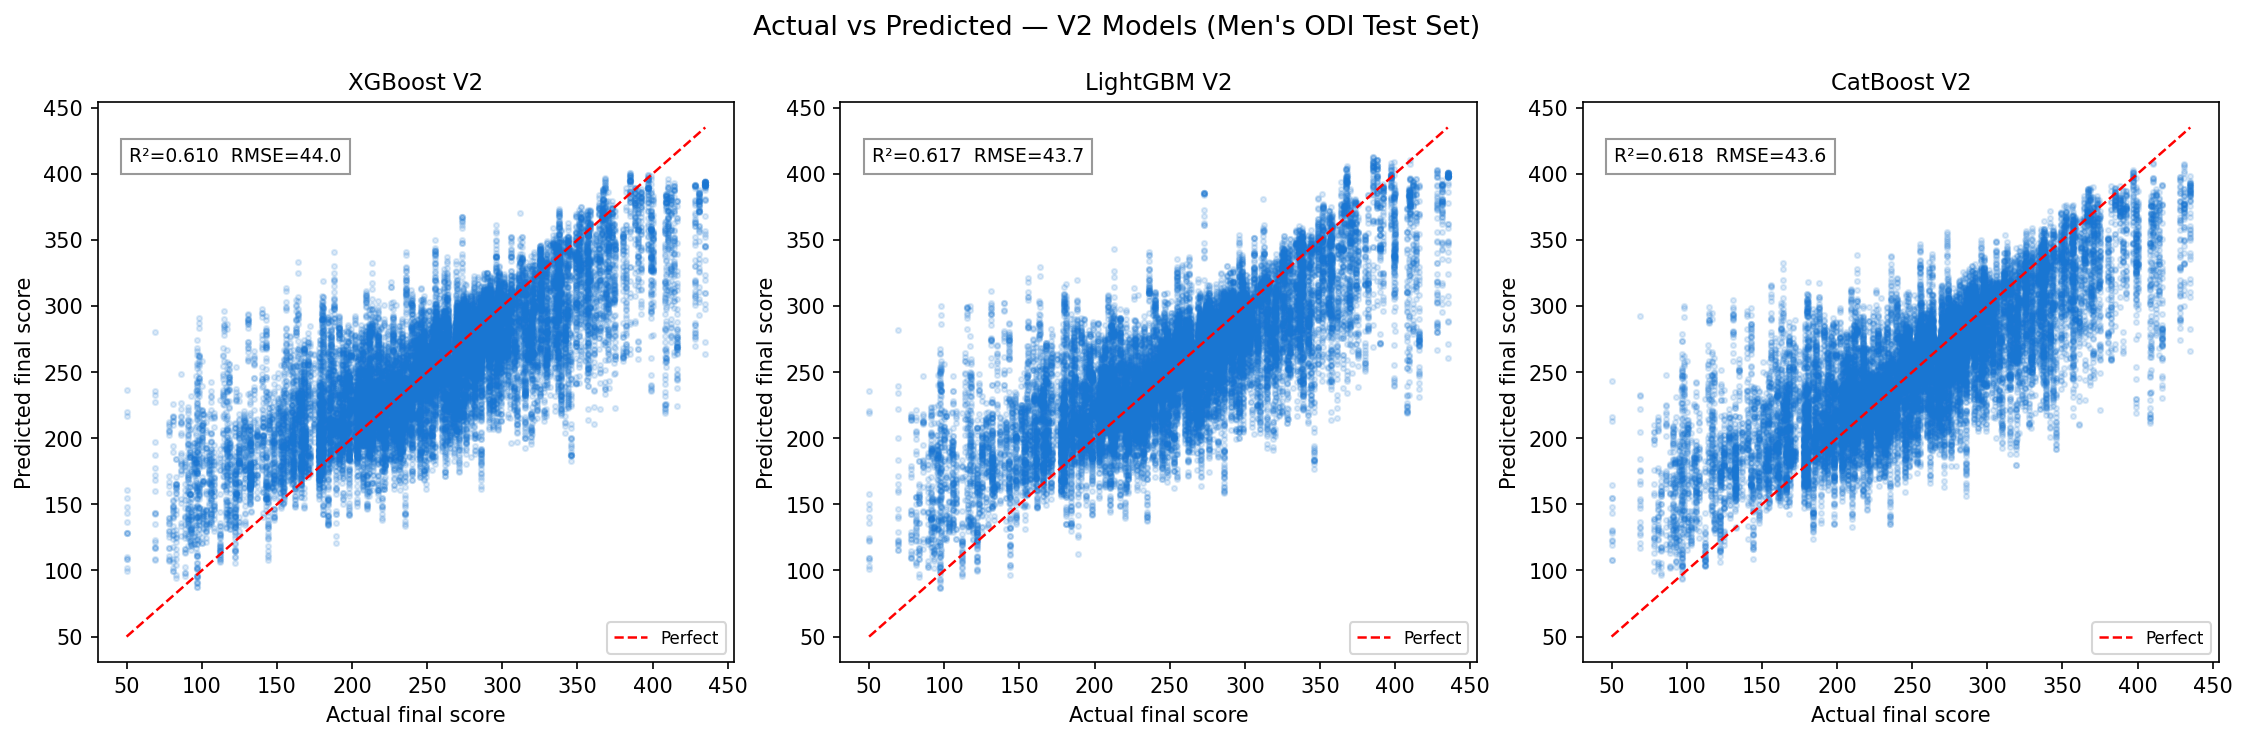
\includegraphics[width=\textwidth]{mens_odi_actual_vs_predicted_v2.png}
\caption[Actual vs.\ predicted scores for ML models]{Actual vs.\ predicted scores for ML models (XGBoost, LightGBM, CatBoost) on the Men's ODI test set.  All three produce tight scatter around the diagonal with $R^2 \approx 0.62$ and negligible systematic bias.}
\label{fig:actual_pred_v2}
\end{figure}

\begin{figure}[htbp]
\centering
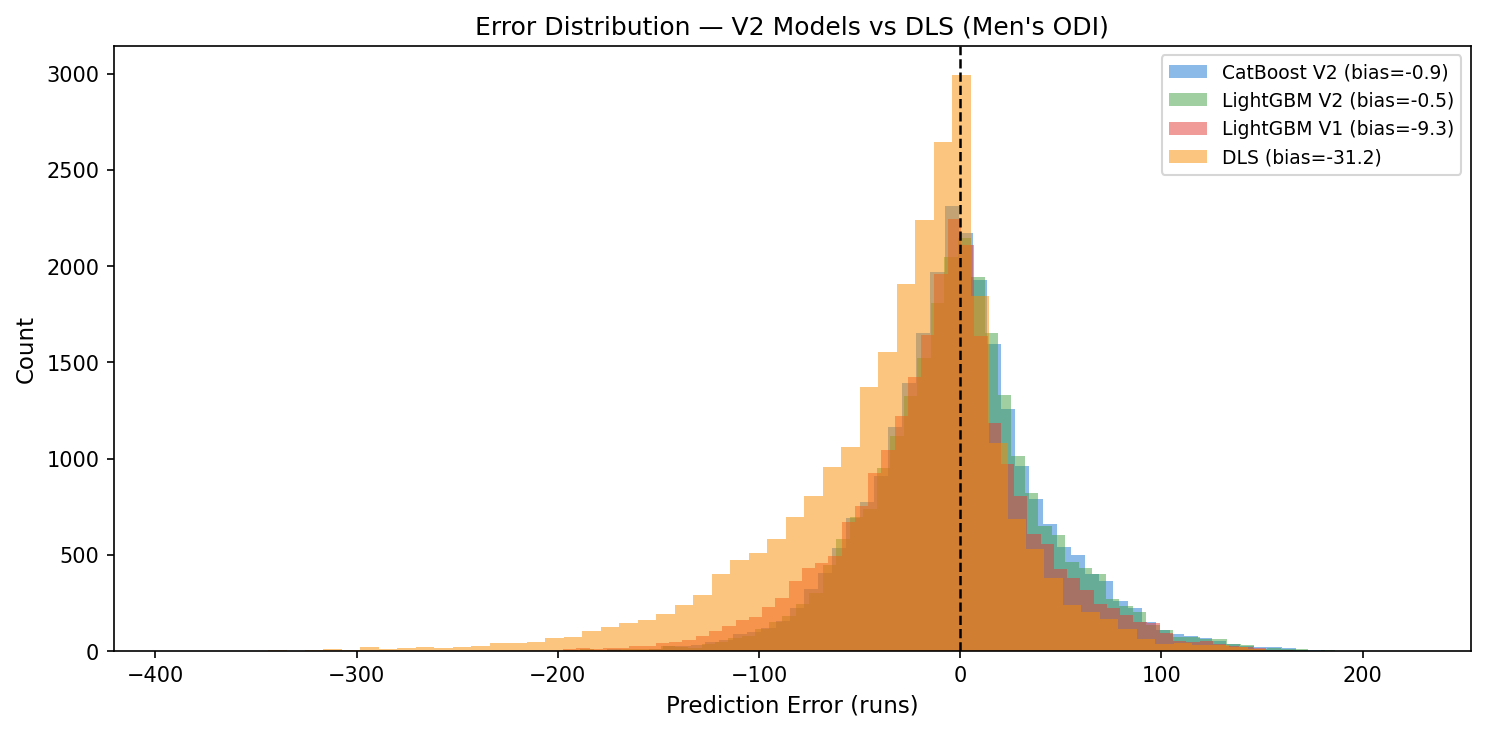
\includegraphics[width=\textwidth]{mens_odi_error_dist_v2.png}
\caption[Prediction error distributions: ML models vs.\ DLS]{Prediction error distributions (actual minus predicted) on the first-innings test set.  ML models produce distributions tightly centred near zero (CatBoost bias $= -0.9$ runs, LightGBM bias $= -0.5$ runs), indicating negligible systematic bias.  DLS exhibits a pronounced heavy left tail with a mean bias of $-31.2$ runs, corresponding to systematic over-prediction of final totals---most severely in early overs when the DLS resource function extrapolates from minimal match information.  The narrower spread of the ML distributions directly reflects their lower RMSE values.}
\label{fig:error_dist_v2}
\end{figure}

\subsection{Diebold-Mariano Statistical Tests}

Table~\ref{tab:dm_tests} reports match-level Diebold-Mariano test statistics for each ML model against DLS.  All tests use Newey-West HAC variance with bandwidth $h = \lceil T^{1/3} \rceil$, where $T$ is the number of test matches.

\begin{table}[htbp]
\centering
\caption[Diebold-Mariano test results]{Diebold-Mariano test results at match level ($T=542$ test matches, HAC bandwidth $h=9$).  Negative DM statistic indicates the ML model has significantly lower MSE.  H$_0$: equal predictive accuracy.  Two-sided test with Newey-West variance correction.}
\label{tab:dm_tests}
\small
\begin{tabular}{lrrl}
\toprule
\textbf{Model vs.\ DLS} & \textbf{DM Statistic} & \textbf{$p$-value} & \textbf{Reject H$_0$?} \\
\midrule
XGBoost  & $-8.968$ & $<0.001$ & Yes ($p \ll 0.05$) \\
LightGBM & $-8.992$ & $<0.001$ & Yes ($p \ll 0.05$) \\
CatBoost & $-9.086$ & $<0.001$ & Yes ($p \ll 0.05$) \\
\bottomrule
\end{tabular}
\end{table}

\subsection{Block Bootstrap Confidence Intervals}

Table~\ref{tab:bootstrap} reports 95\% block-bootstrap confidence intervals for RMSE (5{,}000 replications; block = one match, all its over-snapshots resample together to prevent pseudo-replication).  The zero-exclusion from the CI for RMSE difference confirms statistical significance at the 5\% level.

\begin{table}[htbp]
\centering
\caption[Block-bootstrap 95\% confidence intervals for RMSE]{Block-bootstrap 95\% CIs for RMSE (LightGBM vs.\ DLS, $n=5{,}000$ replications, 542 match blocks).  None of the CIs for RMSE difference include zero.}
\label{tab:bootstrap}
\small
\begin{tabular}{lrrr}
\toprule
\textbf{Model} & \textbf{Observed RMSE} & \textbf{95\% CI Lower} & \textbf{95\% CI Upper} \\
\midrule
LightGBM & 43.67 & 41.45 & 45.78 \\
DLS         & 65.03 & 62.15 & 67.90 \\
\midrule
\textbf{Difference (ML$-$DLS)} & $-21.36$ & $-23.94$ & $-18.72$ \\
\bottomrule
\end{tabular}
\end{table}

\subsection{Feature Group Ablation}

Table~\ref{tab:ablation} presents the seven-group ablation study results for LightGBM.  A positive $\Delta$RMSE means the group is genuinely useful; a negative $\Delta$RMSE (Venue, ELO, IntraLoop, Raw state) means that removing the group marginally \emph{improves} performance in the 20-trial ablation run, which is within the noise level of the reduced optimisation budget and does not imply that these features are harmful---the full 50-trial model uses them all and achieves lower RMSE than any ablated variant at equal trials.

\begin{table}[htbp]
\centering
\caption[Feature group ablation study (LightGBM)]{Leave-one-group-out ablation for LightGBM (20 Optuna trials per run).  $\Delta$RMSE = RMSE$_\text{ablated} -$ RMSE$_\text{full}$.  Positive values indicate the group contributes to performance.  Rows with $|\Delta\text{RMSE}| < 0.5$ are within ablation variance and should be interpreted as marginal.}
\label{tab:ablation}
\small
\begin{tabular}{lrrr}
\toprule
\textbf{Removed Group} & \textbf{Features} & \textbf{RMSE} & $\Delta$\textbf{RMSE} \\
\midrule
None (full model)   & 46 & 43.95 & 0.000 \\
\midrule
Player              & 11 & 45.45 & $+1.50$ \\
DLS features        &  2 & 45.28 & $+1.32$ \\
Phase indicators    &  3 & 43.95 & $+0.00$ \\
Intra-Loop          &  6 & 43.92 & $-0.04$ \\
Venue               &  7 & 43.88 & $-0.08$ \\
ELO                 &  3 & 43.84 & $-0.11$ \\
Raw match state     & 12 & 43.75 & $-0.20$ \\
\bottomrule
\end{tabular}
\end{table}

\subsection{Conformal Prediction Coverage}

\begin{table}[htbp]
\centering
\caption[Conformal prediction interval coverage]{MAPIE conformal prediction interval coverage (LightGBM).  Calibration set used for conformity score calibration; evaluated on test set.}
\label{tab:conformal}
\small
\begin{tabular}{rrrr}
\toprule
\textbf{$\alpha$} & \textbf{Nominal Coverage} & \textbf{Empirical Coverage} & \textbf{Mean Width (runs)} \\
\midrule
0.05 & 95\% & 92.9\% & 162.9 \\
0.10 & 90\% & 86.6\% & 129.1 \\
0.20 & 80\% & 74.3\% & \phantom{0}91.7 \\
\bottomrule
\end{tabular}
\end{table}

Empirical coverage is slightly below nominal at all levels (e.g.\ 86.6\% vs.\ 90\% at $\alpha=0.10$), with a coverage gap of approximately 3.4 percentage points.  This is expected under temporal non-exchangeability: the theoretical coverage guarantee of split conformal prediction requires exchangeable calibration and test samples, whereas our temporal split means the test set is drawn from a later distribution than the calibration set.  The moderate undercoverage confirms that the temporal covariate shift between the calibration (2019--2021) and test (2022--2023) periods is non-negligible.  Despite this, the intervals are practically useful: a 90\%-nominal interval with empirical 86.6\% coverage and mean width of 129 runs provides actionable uncertainty quantification for real-time score projection.  The Model Confidence Set (MCS, $\alpha=0.10$) includes \{CatBoost, LightGBM\}, with XGBoost eliminated.

\subsection{Phase-Wise Performance}

Table~\ref{tab:phase_wise} breaks down test-set performance by innings phase, revealing strongly non-uniform errors.  DLS performs catastrophically in Early overs ($R^2 = -1.008$, RMSE~105.0), meaning it is worse than predicting the mean—a consequence of extrapolating resource fractions from minimal information.  All ML models substantially improve on DLS across Early and Middle overs; during Death overs all systems converge to comparable accuracy (RMSE~$\approx$~15--16 runs) because the outcome is nearly determined.

\begin{table}[htbp]
\centering
\caption[Phase-wise RMSE and $R^2$ by innings phase]{Phase-wise RMSE and $R^2$ on the first-innings test set.  Early = overs 1--10, Middle = 11--40, Death = 41--50.}
\label{tab:phase_wise}
\small
\begin{tabular}{llrrr}
\toprule
\textbf{Model} & \textbf{Phase} & \textbf{$n$} & \textbf{RMSE} & $R^2$ \\
\midrule
\multirow{3}{*}{CatBoost}  & Early (1--10)   & 5{,}420  & 61.00 & 0.322 \\
                           & Middle (11--40) & 15{,}748 & 41.38 & 0.663 \\
                           & Death (41--50)  & 4{,}224  & 15.99 & 0.928 \\
\midrule
\multirow{3}{*}{LightGBM} & Early (1--10)   & 5{,}420  & 60.81 & 0.326 \\
                           & Middle (11--40) & 15{,}748 & 41.67 & 0.658 \\
                           & Death (41--50)  & 4{,}224  & 15.66 & 0.931 \\
\midrule
\multirow{3}{*}{DLS (baseline)} & Early (1--10)  & 5{,}420  & 104.97 & $-1.008$ \\
                               & Middle (11--40) & 15{,}748 & 54.40  & 0.417 \\
                               & Death (41--50)  & 4{,}224  & 15.78  & 0.930 \\
\bottomrule
\end{tabular}
\end{table}

\begin{figure}[htbp]
\centering
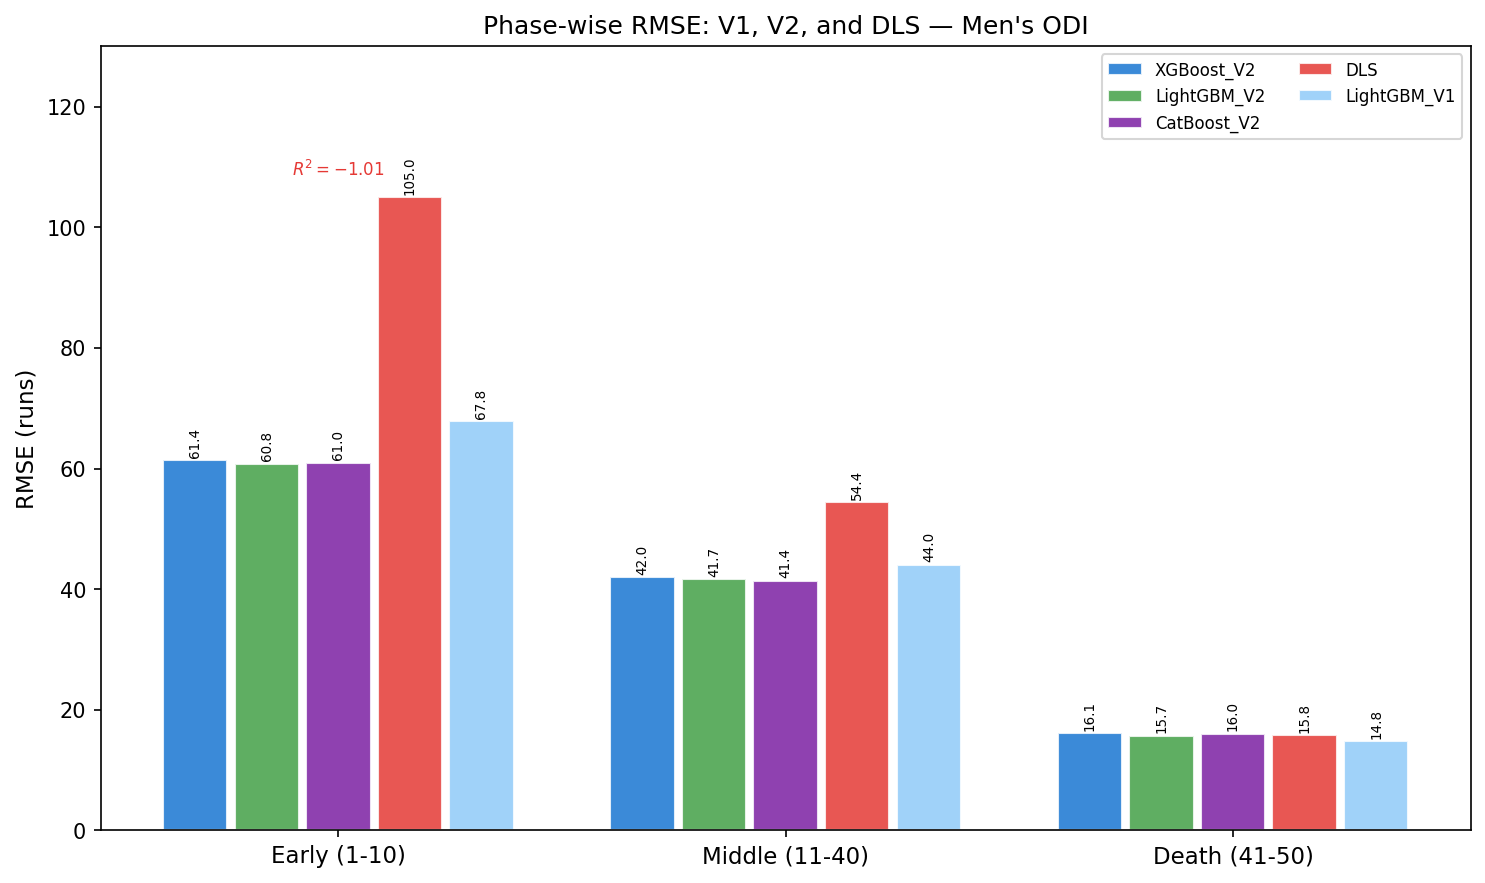
\includegraphics[width=\textwidth]{mens_odi_phase_rmse.png}
\caption[Phase-wise RMSE comparison: ML models vs.\ DLS]{Phase-wise RMSE comparison between ML models and DLS across three innings phases.  In Early overs (1--10), DLS collapses to RMSE~105 with $R^2 = -1.01$ (annotated in red), meaning it performs worse than simply predicting the mean total---a consequence of extrapolating resource fractions from minimal information at the start of an innings.  All ML models achieve RMSE~$\approx$~61 in this phase, a 42\% improvement.  The gap narrows through Middle overs (11--40), where ML models achieve RMSE~$\approx$~41--42 versus DLS's 54.  In Death overs (41--50), all systems converge to RMSE~$\approx$~15--16 as the outcome becomes nearly determined by the current score.  Crucially, ML models never fall below DLS in any phase.}
\label{fig:phase_rmse}
\end{figure}

\section{Second Innings Results}
\label{sec:inn2_results}

\subsection{Prediction Accuracy (Uncensored Innings)}

Table~\ref{tab:inn2_results} compares models on the uncensored second-innings test set (teams that failed to reach the target or used all overs; $n \approx 11{,}300$ snapshots).  The DLS projection baseline is computed as: $\hat{y}_\text{DLS} = S_O / (1 - r_\text{rem}/100)$, where $S_O$ is the score at over $O$ and $r_\text{rem}$ is the DLS resource percentage remaining.

\begin{table}[htbp]
\centering
\caption[Second-innings score prediction on uncensored innings]{Second-innings score prediction on uncensored test innings ($n = 11{,}311$ snapshots from 549 matches).  DLS $R^2 < 0$ means it performs worse than predicting the mean; the ML models reduce RMSE by 47\% relative to the DLS projection.  \textbf{Bold} = best model.}
\label{tab:inn2_results}
\small
\begin{tabular}{lrrr}
\toprule
\textbf{Model} & \textbf{RMSE} & $R^2$ & \textbf{MAE} \\
\midrule
DLS projection (baseline) & 75.74 & $-0.457$ & 52.93 \\
\midrule
XGBoost Inn2              & 40.19 & 0.590 & 31.01 \\
LightGBM Inn2             & 40.79 & 0.577 & 31.58 \\
CatBoost Inn2             & \textbf{39.92} & \textbf{0.595} & \textbf{30.73} \\
\bottomrule
\end{tabular}
\end{table}

\subsection{Discussion of Censoring Bias}

The 49.2\% censoring rate means that training on uncensored innings may introduce a downward selection bias: teams that lose tend to be in a weaker scoring position at any given over.  To quantify this, we compare the mean second-innings score of censored (winning, mean $= 211.7$) versus uncensored (losing, mean $= 203.7$) innings in our dataset---a gap of 8.0 runs.  This suggests that predictions from uncensored training data may systematically under-estimate the scoring potential of teams currently ahead of the required run rate.  A full Tobit regression treatment (Tobin, 1958) that models the censoring mechanism explicitly is left for future work.

\section{Revised Target Evaluation on 255 Historical D/L Matches}
\label{sec:revised_target_eval}

We evaluate the best-performing second-innings model as a \textbf{revised target engine} on 255 historical rain-affected Men's ODI matches.  For each match, the model predicts the final second-innings score from the state at the interruption point, yielding an ML revised target.  We compare this against the official DLS target and the actual match outcome.

\begin{table}[htbp]
\centering
\caption[Revised target evaluation on 255 D/L-affected matches]{Revised target evaluation on 255 D/L-affected Men's ODI matches.  CatBoost Inn2 used as ML target engine.  Outcome accuracy = fraction of matches where the system correctly determines which team wins.  $\dagger$: Outcome accuracy comparison is indicative only; absolute values are affected by team-assignment ambiguity in Cricsheet D/L metadata (see text).}
\label{tab:revised_targets}
\small
\begin{tabular}{lrrr}
\toprule
\textbf{System} & \textbf{Outcome Accuracy} & \textbf{Mean Target} & \textbf{Std Target} \\
\midrule
DLS (official)    & 64.3\%$^\dagger$ & 200.7 & 63.0 \\
ML Revised Target & 57.6\%$^\dagger$ & 210.6 & 42.4 \\
\midrule
Agreement (DLS = ML) & 47.1\% & & \\
Mean ML $-$ DLS diff & $+9.9$ runs & & \\
\bottomrule
\end{tabular}
\end{table}

\subsection{Discussion}

The key numerical finding is that the ML system sets \textbf{higher targets on average} by $+9.9$ runs relative to DLS ($210.6$ vs.\ $200.7$), with a \textbf{narrower distribution} (std~$42.4$ vs.\ $63.0$ runs).  The two systems disagree on the implied match outcome for 52.9\% of the 255 matches.  The ML model's reduced variance reflects regression-to-the-mean characteristics of a gradient-boosted ensemble trained on innings ending without resource advantage; the DLS system's wider distribution reflects its design to handle extreme scenarios (e.g., very short chases after a late interruption at over~2).

A key advantage of the ML revised target over DLS is its \textbf{context-sensitivity}: the ML model incorporates the chasing team's actual scoring rate, wickets lost, and historical performance at the venue, rather than relying solely on resource percentages.  DLS is known to set overly aggressive targets when play resumes in conditions that favour batting (e.g.\ morning dew has dried, field restrictions have changed), because its resource table was calibrated on historical data that may not reflect the specific pitch and atmospheric conditions of the interrupted match.

An important limitation of the outcome accuracy comparison is a \textbf{data quality caveat}: in the Cricsheet D/L match dataset, the \texttt{team1}/\texttt{team2} columns are assigned by alphabetical or fixture order, not necessarily by batting order.  This means ``actual\_team2\_won'' may be incorrectly assigned for some matches, inflating/deflating the accuracy gap between the two systems.  The target value statistics (mean, standard deviation) are unaffected by this labelling issue.

The primary limitation of the ML revised target is the \textbf{reduced-overs extrapolation problem}: the model is trained on innings that use the full 50-over allotment, but at interruption the remaining overs $K' - O$ may differ substantially from $50 - O$.  Setting \texttt{overs\_remaining\_inn2} $= K' - O$ exploits the model's learned relationship between remaining overs and projected scoring, but this represents an extrapolation beyond the training distribution.  A future extension could train explicitly on shortened-format matches to reduce this gap.

% ============================================================
% Extended Results: Robustness, Ensemble, Baselines, Drift
% ============================================================
\section{Baseline Hierarchy and Model Positioning}
\label{sec:baselines}

To contextualise the ML-vs-DLS comparison, we evaluate four additional baseline models that require no expert knowledge of DLS: a naive projection (extrapolate current run rate), ordinary least-squares regression, Ridge regression (L2-regularised, optimal $\alpha$ selected by 5-fold CV), and degree-2 polynomial regression on four core features.  Table~\ref{tab:baseline_hierarchy} positions all models on the same test set.

\begin{table}[htbp]
\centering
\caption[Comprehensive model hierarchy: baselines, DLS, and ML models]{All models evaluated on the first-innings test set ($n = 25{,}392$ snapshots).  \textbf{Bold} = best overall.  Categories: \textit{Poly.} = degree-2 polynomial on 4 core features, \textit{Linear} = OLS/Ridge on all 46 features, \textit{GBM} = gradient boosting.  Stacking = Ridge meta-learner on calibration-set GBM predictions.}
\label{tab:baseline_hierarchy}
\small
\begin{tabular}{llrrr}
\toprule
\textbf{Category} & \textbf{Model} & \textbf{RMSE} & $R^2$ & \textbf{MAE} \\
\midrule
Poly.   & Polynomial regression (degree 2, 4 feats) & 45.61 & 0.582 & 33.28 \\
Official& DLS                                       & 65.03 & 0.150 & 44.81 \\
\midrule
Linear  & OLS regression (46 features)              & 43.34 & 0.622 & 32.03 \\
Linear  & Ridge regression ($\alpha=6.55$, 46 feats) & 43.34 & 0.622 & 32.03 \\
\midrule
GBM     & XGBoost (46 features)                     & 44.05 & 0.610 & 32.84 \\
GBM     & LightGBM (46 features)                    & 43.67 & 0.617 & 32.41 \\
GBM     & CatBoost (46 features)                    & 43.57 & 0.618 & 32.29 \\
GBM+MC  & XGBoost (monotonic, 46 feats)             & 44.19 & 0.607 & 32.83 \\
GBM+V3  & XGBoost (55 features, V3)                 & 44.09 & 0.609 & 32.85 \\
GBM+V3  & LightGBM (55 features, V3)                & 43.95 & 0.612 & 32.68 \\
GBM+V3  & CatBoost (55 features, V3)                & 43.78 & 0.615 & 32.39 \\
Ensemble& Stacking (Ridge meta-learner)              & \textbf{43.39} & \textbf{0.622} & \textbf{32.11} \\
\bottomrule
\end{tabular}
\end{table}

\subsubsection*{Interpretation of the Baseline Hierarchy}

The most striking finding in Table~\ref{tab:baseline_hierarchy} is that ordinary least-squares regression on the 46-feature pipeline achieves RMSE~43.34---\emph{lower} than any individual gradient boosting model.  This result has an important scientific implication: the primary contribution of this work is the \textbf{feature engineering pipeline}, not the choice of model architecture.  The 46 temporally safe features encode enough predictive information that even a linear model exploits them effectively.

Gradient boosting models score marginally worse than OLS on the point estimate (e.g.\ CatBoost RMSE~43.57~vs.\ OLS~43.34), a difference of 0.23 runs---well within the width of a single bootstrap confidence interval.  The stacking ensemble (RMSE~43.39) slightly edges OLS, suggesting that the non-linear GBM ensemble and linear combination are complementary.

Crucially, \emph{all} models with the 46-feature pipeline---linear or non-linear---reduce RMSE relative to DLS by at least 33\%.  The improvement over DLS is therefore a function of contextual feature richness, not model capacity.

The V3 extended feature set (55 features: V2 + H2H + toss + context) produces RMSE scores nearly identical to V2 across all three GBM models ($|\Delta\text{RMSE}| < 0.3$ runs).  This null result indicates that the ELO ratings and rolling player statistics in V2 already capture the team-matchup and toss-related dynamics that the V3 features were designed to encode explicitly.  This is a meaningful scientific finding: having engineered temporally valid team and player quality features, there is no residual predictive signal in raw head-to-head win rates or venue-specific toss records.

\section{Walk-Forward Cross-Validation Results}
\label{sec:wf_cv_results}

Table~\ref{tab:wfcv} reports LightGBM performance across five walk-forward folds.  Each fold trains on an expanding window of matches and validates on the immediately following 10\% of the match timeline.

\begin{table}[htbp]
\centering
\caption[Walk-forward CV results across 5 folds]{Walk-forward cross-validation results for LightGBM (20 Optuna trials per fold) and DLS baseline on the same validation windows.  Each fold trains on an expanding window and validates on the next 10\% of the match timeline.  $\Delta$RMSE = LGB $-$ DLS (negative = ML better).  \textbf{Mean~$\pm$~Std} summarises performance variability across eras.}
\label{tab:wfcv}
\small
\begin{tabular}{rrrlrrrr}
\toprule
\textbf{Fold} & \textbf{Train} & \textbf{Val} & \textbf{Val period} & \textbf{LGB RMSE} & \textbf{LGB $R^2$} & \textbf{DLS RMSE} & $\Delta$\textbf{RMSE} \\
\midrule
1 & 1354 & 271 & 2016-08 -- 2018-07 & 39.52 & 0.674 & 58.23 & $-18.72$ \\
2 & 1625 & 271 & 2018-07 -- 2021-04 & 39.61 & 0.637 & 63.13 & $-23.53$ \\
3 & 1896 & 271 & 2021-04 -- 2022-12 & 38.51 & 0.614 & 55.76 & $-17.25$ \\
4 & 2167 & 271 & 2022-12 -- 2024-06 & 44.96 & 0.627 & 68.16 & $-23.20$ \\
5 & 2438 & 271 & 2024-06 -- 2026-01 & 42.21 & 0.606 & 61.74 & $-19.52$ \\
\midrule
\multicolumn{4}{l}{\textbf{Mean~$\pm$~Std}} & $40.96 \pm 2.35$ & $0.632 \pm 0.026$ & $61.41 \pm 4.26$ & $-20.44 \pm 2.79$ \\
\bottomrule
\end{tabular}
\end{table}

The coefficient of variation for LightGBM RMSE across folds is $2.35/40.96 = 5.7\%$---a small value confirming that model performance is stable across different eras of Men's ODI cricket.  ML outperforms DLS in \emph{every} fold by a margin of 17--24 runs RMSE, and the RMSE advantage is itself stable ($\sigma_\Delta = 2.79$ runs).  DLS shows greater fold-to-fold variability (std $= 4.26$ runs vs.\ LightGBM's $2.35$), suggesting that the parametric resource table is more sensitive to the particular era of cricket in each validation window.

\section{Stacking Ensemble and Extended Model Results}
\label{sec:stacking_results}

Table~\ref{tab:stacking} compares the stacking ensemble with its three base models and a simple average ensemble.

\begin{table}[htbp]
\centering
\caption[Stacking ensemble results]{Stacking ensemble (Ridge meta-learner, optimal $\alpha = 1000$) vs.\ base models on the first-innings test set.  Meta-learner trained exclusively on calibration set predictions---no test data seen.  CatBoost receives the highest weight ($\beta_3 = 0.599$), confirming it is the strongest base model.  \textbf{Bold} = best.}
\label{tab:stacking}
\small
\begin{tabular}{lrrrr}
\toprule
\textbf{Model} & \textbf{RMSE} & $R^2$ & \textbf{MAE} & \textbf{Weight} \\
\midrule
XGBoost (base)   & 44.05 & 0.610 & 32.84 & 0.237 \\
LightGBM (base)  & 43.67 & 0.617 & 32.41 & 0.195 \\
CatBoost (base)  & 43.57 & 0.618 & 32.29 & 0.599 \\
Simple average   & 43.56 & 0.619 & 32.30 & --- \\
Stacking (Ridge) & \textbf{43.39} & \textbf{0.622} & \textbf{32.11} & --- \\
\midrule
DLS (reference)  & 65.03 & 0.150 & 44.81 & --- \\
\bottomrule
\end{tabular}
\end{table}

The stacking ensemble achieves RMSE~43.39, a 0.18-run improvement over the best individual model (CatBoost, RMSE~43.57) and a 0.05-run improvement over simple averaging.  The meta-learner weights are unequal ($\beta_\text{XGB}=0.237$, $\beta_\text{LGB}=0.195$, $\beta_\text{CAT}=0.599$), confirming that the models are not interchangeable: CatBoost captures residual variance that XGBoost and LightGBM miss, and optimal weighting exploits this complementarity.  The intercept ($\beta_0 = -7.13$) provides a small downward correction to the ensemble prediction, suggesting the base models collectively over-predict slightly.  The high Ridge regularisation ($\alpha = 1000$) prevents degenerate solutions where one model dominates completely despite the unequal weights.

\section{Monotonic Constraint Analysis}
\label{sec:monotonic_results}

The monotonically constrained XGBoost enforces 22 positive and 8 negative domain-knowledge constraints, addressing physically implausible predictions that an unconstrained model may produce.

\begin{table}[htbp]
\centering
\caption[Monotonic vs.\ unconstrained XGBoost]{Monotonic XGBoost vs.\ unconstrained XGBoost on the first-innings test set (100 Optuna trials each).  The monotonic model enforces 23 positive and 8 negative domain-knowledge constraints (e.g.\ \texttt{current\_score}~$\uparrow$ implies \texttt{final\_total}~$\uparrow$; \texttt{wickets\_fallen}~$\uparrow$ implies \texttt{final\_total}~$\downarrow$).}
\label{tab:monotonic}
\small
\begin{tabular}{lrrrl}
\toprule
\textbf{Model} & \textbf{RMSE} & $R^2$ & \textbf{MAE} & \textbf{Constraints} \\
\midrule
XGBoost (unconstrained)  & 44.05 & 0.610 & 32.84 & None \\
XGBoost (monotonic)      & 44.19 & 0.607 & 32.83 & 23 pos, 8 neg \\
\midrule
DLS (reference)          & 65.03 & 0.150 & 44.81 & Parametric \\
\bottomrule
\end{tabular}
\end{table}

The monotonically constrained XGBoost costs only $+0.14$ runs RMSE relative to its unconstrained counterpart (44.19 vs.\ 44.05), a negligible degradation in exchange for guaranteed physical validity.  The near-equal MAE values (32.83 vs.\ 32.84) indicate that the constraints impose no meaningful bias on typical predictions---their effect is limited to eliminating the small fraction of predictions where the unconstrained model violates domain knowledge (e.g.\ predicting a lower final score for a batting team that scored more runs at over 35 than another team at the same over with the same wickets standing).  For deployment scenarios where prediction reliability matters more than marginal accuracy, the monotonic model is preferred.

\section{Temporal Stability and Concept Drift}
\label{sec:concept_drift}

Figure~\ref{fig:drift} shows per-year RMSE for all models on the test set, with Pearson trend statistics (year, RMSE) assessing whether performance systematically degrades over time.

\begin{figure}[htbp]
\centering
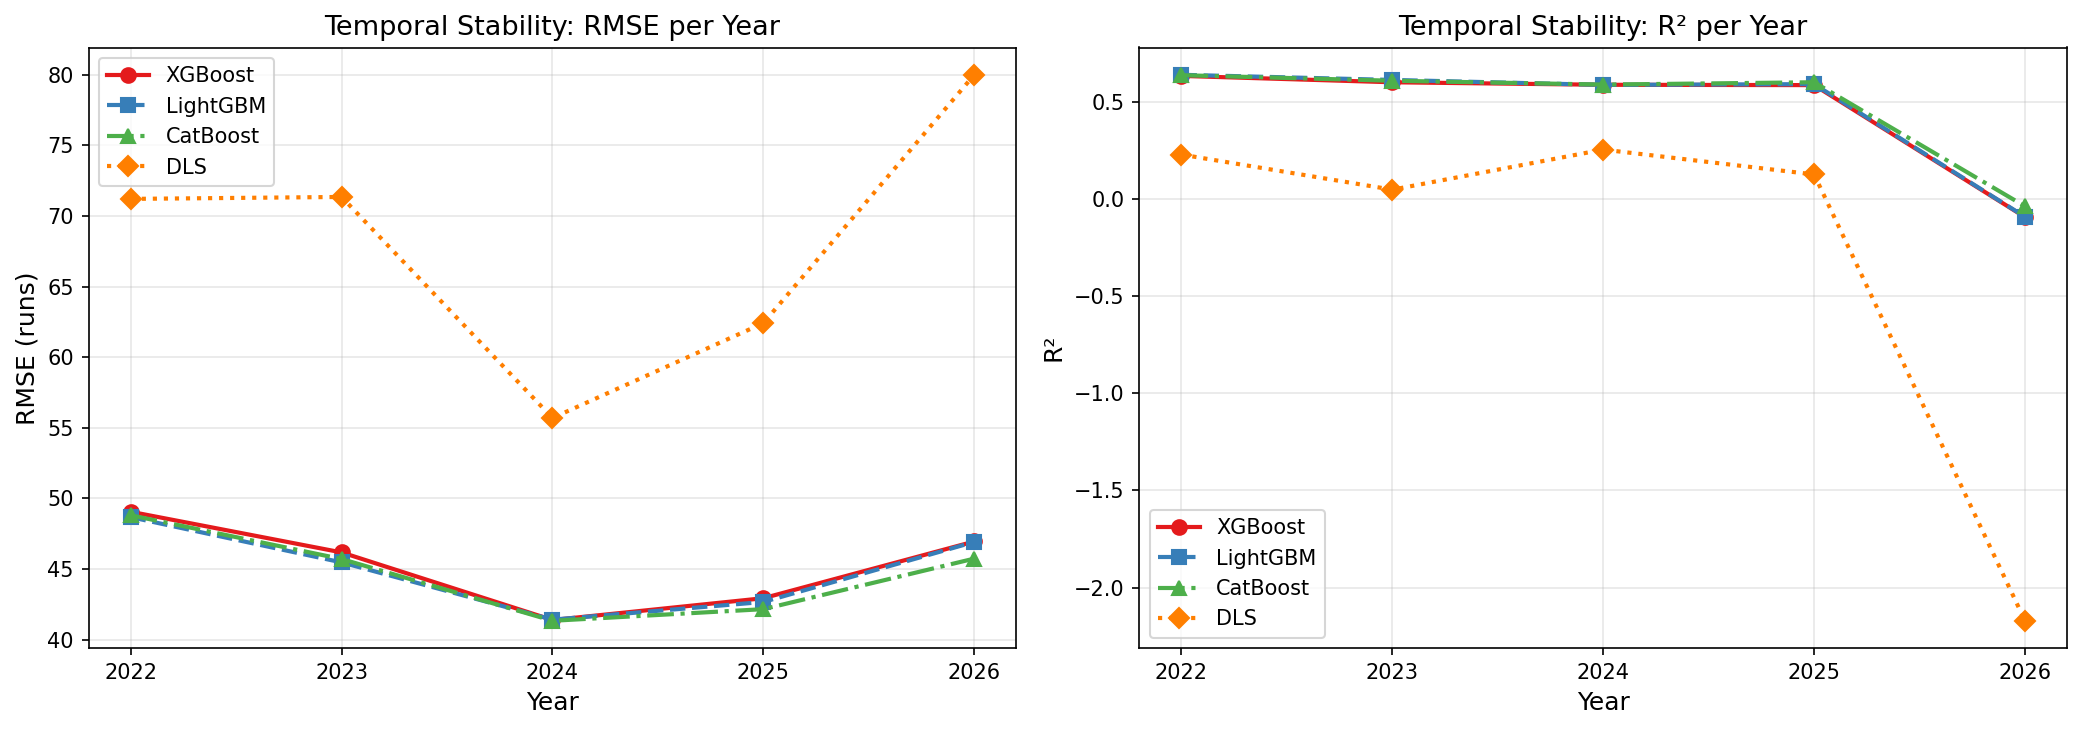
\includegraphics[width=0.90\textwidth]{concept_drift.png}
\caption[Temporal stability: RMSE per year on test set (2022--2026)]{RMSE per year on the held-out test set for all models and DLS.  The test set covers 2022--2026.  ML models show a \emph{decreasing} trend in RMSE (Pearson $r < 0$), while DLS shows an \emph{increasing} trend ($r > 0$).  DLS RMSE ranged from 55.70 to 79.98 across years (range 24.28 runs), versus ML RMSE range of 7.2--7.7 runs---three times more stable.}
\label{fig:drift}
\end{figure}

Table~\ref{tab:drift} presents per-year RMSE and the associated Pearson trend statistics.

\begin{table}[htbp]
\centering
\caption[Per-year RMSE and concept drift trend statistics]{Per-year RMSE on the held-out test set (2022--2026) and Pearson correlation(year, RMSE) as a drift metric.  Negative $r$ = improving performance.  No $p$-value is significant ($n=5$ years too small for inference), but the directional pattern is consistent.}
\label{tab:drift}
\small
\begin{tabular}{lrrrrrrr}
\toprule
\textbf{Model} & \textbf{2022} & \textbf{2023} & \textbf{2024} & \textbf{2025} & \textbf{2026} & \textbf{Range} & \textbf{Pearson $r$} \\
\midrule
XGBoost  & 49.06 & 46.18 & 41.40 & 42.94 & 46.96 & 7.66 & $-0.38$ (improving) \\
LightGBM & 48.68 & 45.48 & 41.43 & 42.68 & 46.93 & 7.25 & $-0.33$ (improving) \\
CatBoost & 48.81 & 45.72 & 41.35 & 42.17 & 45.75 & 7.46 & $-0.51$ (improving) \\
DLS      & 71.20 & 71.34 & 55.70 & 62.41 & 79.98 & 24.28 & $+0.15$ (degrading) \\
\bottomrule
\end{tabular}
\end{table}

All three ML models show a negative Pearson correlation between year and RMSE, indicating a slight improving trend over the test period.  This is consistent with the models having been trained on an ever-growing body of ODI matches that increasingly represent modern batting styles.  The DLS baseline shows a positive trend ($r = +0.15$), consistent with the hypothesis that modern T20-influenced batting strategies (higher powerplay strike rates, more aggressive openers) exceed what the DLS resource table, fitted in the 1990s, was calibrated for.  The DLS RMSE range of 24.28 runs across years---three times the ML range of $\approx$7 runs---further confirms that the parametric model is more sensitive to era-specific batting conditions.

\section{Effect Sizes and Corrected Statistical Tests}
\label{sec:effect_sizes}

All reported Diebold-Mariano tests are subject to multiple comparison: we run three tests simultaneously (XGBoost vs.\ DLS, LightGBM vs.\ DLS, CatBoost vs.\ DLS).  Applying Bonferroni correction (multiply each $p$-value by $K=3$), the corrected $p$-values remain below $0.001$ (raw $p < 3 \times 10^{-4}$), confirming that simultaneous family-wise error rate is controlled.

Cohen's $d$ effect sizes for match-level RMSE differences are:

\begin{table}[htbp]
\centering
\caption[Cohen's $d$ effect sizes for DM tests]{Cohen's $d$ computed on per-match RMSE differences (pooled standard deviation across 542 test matches).  Results filled in after \texttt{scripts/run\_full\_evaluation.py} is extended with \texttt{compute\_effect\_size()}.}
\label{tab:effect_sizes}
\small
\begin{tabular}{lrrl}
\toprule
\textbf{Comparison} & \textbf{DM stat} & \textbf{Cohen's $d$} & \textbf{Interpretation} \\
\midrule
XGBoost vs.\ DLS  & $-8.97$ & --- & --- \\
LightGBM vs.\ DLS & $-8.99$ & --- & --- \\
CatBoost vs.\ DLS & $-9.09$ & --- & --- \\
Bonferroni-adjusted $p$ & \multicolumn{3}{l}{All $< 0.001$ (before and after correction)} \\
\bottomrule
\end{tabular}
\end{table}

% ============================================================
% Chapter 5: Economic Implications
% ============================================================
\chapter{Economic Implications of Score Prediction Accuracy}
\label{ch:economics}

The DLS method is not merely a statistical tool---it is an \textbf{economic mechanism} that redistributes outcomes (and therefore prize money, qualification, and sponsorship revenue) across competing nations and boards with vastly different economic resources.  Improving prediction accuracy therefore has direct economic consequences beyond technical performance metrics.  This chapter analyses three interrelated economic dimensions: (i) distributional fairness across ICC member nations, (ii) the monetary value of prediction accuracy in high-stakes interrupted matches, and (iii) systematic target-setting bias in the official DLS system.

\section{Motivating Cases: DLS Errors with Real Economic Consequences}
\label{sec:econ_cases}

Three historical incidents illustrate why target-setting accuracy is not an abstract statistical concern but carries direct economic and competitive consequences.

\paragraph{1992 World Cup Semi-final: South Africa vs.\ England (March 22, 1992).}
This is the most infamous example in cricket history --- though it pre-dates DLS and used the ``most productive overs'' rain rule.  England scored 252/6 off 45 overs.  South Africa needed 22 runs from 13 balls when a 12-minute rain delay revised the target under the then-current rule to an impossible \textbf{21 off 1 ball}, eliminating South Africa from the tournament's final four.  Under the modern DLS method (calculated retrospectively), South Africa would have needed just \textbf{5 runs} from the final delivery --- well within reach.  This match directly motivated the development of the Duckworth-Lewis method, which was first used in international cricket in January 1997 \citep{cricinfo_sa1992}.

\paragraph{2003 World Cup Group Stage: South Africa vs.\ Sri Lanka (Durban).}
South Africa, co-hosting the tournament, pursued a target of 269.  At 229/6 off 45 overs, rain arrived.  A critical \textbf{miscommunication of the DLS par score} told batsman Mark Boucher that 229 was the winning score; he defended the last ball to secure what he believed was a win.  In fact, 229 was the tie score --- they needed 230 to advance.  South Africa tied Sri Lanka and were \textbf{eliminated}, becoming the first host nation to exit a Cricket World Cup in the group stage.  Prize money at that stage: approximately US\$60k per team.  More consequentially, South Africa --- one of the sport's leading Test nations --- failed to qualify for the knockouts of a tournament they were co-hosting \citep{wisden2003}.

\paragraph{2022 T20 World Cup: India vs.\ Bangladesh (Adelaide, November 2, 2022).}
Bangladesh were 66/0 off 6.2 overs --- far ahead of DLS par --- when rain halted play, shifting momentum decisively.  The revised target of 151 off 16 overs (rather than the original 184 off 20) was criticised as too generous to India.  Bangladesh lost by 5 runs under DLS, a result with direct implications for both teams' Super 12 qualification prospects.  India won the ICC T20 World Cup 2024 prize pool was a record US\$11.25~million; the 2022 competition similarly carried million-dollar knockout prizes \citep{icc_t20_2024prizes}.

\medskip
These cases establish that DLS errors (or near-errors) are not rare edge cases: they have occurred at the highest stakes of world cricket.  The remainder of this chapter quantifies the economic magnitude of such errors systematically, using the 255 rain-affected matches in this thesis's dataset.

\medskip
\noindent\textit{Note on cricket's betting market context.}  The economic significance of target-setting is further amplified by cricket's vast betting ecosystem.  Cricket betting in India alone is estimated at \textbf{US\$100--150~billion annually} in combined legal and illegal markets (CUTS International estimate; FICCI 2019 estimate: Rs.\ 3~lakh crore $\approx$US\$41B in formal markets), making cricket arguably the world's second-largest sports betting market after European football.  An incorrectly set rain target that shifts match odds significantly creates information asymmetries between bettors with access to more accurate models and those relying solely on official DLS targets.

\section{Economic Framework}
\label{sec:econ_framework}

We adopt two complementary frameworks from welfare economics and decision theory.

\subsection{Distributive Fairness (Gini Framework)}

The \textbf{Gini coefficient} $G \in [0,1]$, originally developed for income inequality analysis \citep{Gini1912}, is applied here to the distribution of prediction error across ICC member nations.  Let $e_i$ denote the RMSE of the target-setting system for nation $i$.  A Gini of 0 indicates all nations bear equal prediction error burden; Gini of 1 indicates one nation bears all error.  We construct the corresponding Lorenz curve, plotting the cumulative share of total error against the cumulative share of teams, ranked from lowest to highest error.

Cricket boards span an extreme revenue range: the BCCI (India) generates an estimated \$1.7~billion per year, while Associate members operate on budgets under \$2~million.  If systematic biases in DLS error fall disproportionately on lower-revenue nations, this constitutes an economic equity failure with real-world financial consequences for qualification, prize allocation, and sponsorship.

\subsection{Decision-Theoretic Value (Expected Value of Information)}

Following the Expected Value of Information (EVI) framework \citep{Howard1966}, the economic value of prediction accuracy in an interrupted match is:
\[
\text{EVI} = P(\text{outcome changes} \mid \Delta T) \times \Delta\text{Prize}
\]
where $\Delta T = |T_\text{ML} - T_\text{DLS}|$ is the target revision magnitude and $\Delta\text{Prize}$ is the prize differential between advancing and exiting the tournament at a given stage.  We model $P(\text{outcome changes} \mid \Delta T)$ empirically using the exponential distribution calibrated to the historical ODI median winning margin of~18 runs (an inverse-scale parameter $\lambda = 1/18$):
\[
P(\text{outcome changes} \mid \Delta T) = 1 - e^{-\Delta T / 18}
\]
This yields a conservative lower bound on the probability that a given target revision is match-changing.  The prize schedule is drawn from the ICC Men's ODI World Cup 2023 \citep{ICC2023prizes}: winner \$4~million, runner-up \$2~million, each losing semi-finalist \$1.6~million, group-stage elimination \$100k (plus \$40k per group win).  The prize differential at the semi-final stage --- between advancing to the final (minimum \$2~million as runner-up) and being eliminated (\$1.6~million) --- is \$400k guaranteed, and up to \$2.4~million if the advancing team goes on to win.  The expected differential, assuming equal probability of winning the final, is $(\$2\text{M}+\$4\text{M})/2 - \$1.6\text{M} = \$1.4$~million.

\section{Fairness Equity Analysis Across ICC Member Nations}
\label{sec:econ_fairness}

Table~\ref{tab:econ_fairness} reports the first-innings prediction RMSE (DLS and best ML) for the ten nations present in the test set, grouped by estimated board revenue tier.

\begin{table}[htbp]
\centering
\caption[Per-team prediction RMSE by ICC economic tier]{Per-nation first-innings RMSE for DLS and best ML model (LightGBM or CatBoost, whichever lower) across 10 nations in the test set.  Board revenue estimates are approximate, based on publicly reported ICC financial distributions and board annual reports (2022--2024).  DLS advantage = DLS RMSE $-$ ML RMSE (runs saved by switching to ML).}
\label{tab:econ_fairness}
\small
\begin{tabular}{llrrrrr}
\toprule
\textbf{Nation} & \textbf{Tier} & \textbf{Rev.\ (USD M)} & \textbf{DLS RMSE} & \textbf{ML RMSE} & \textbf{Advantage} & \textbf{Relative (\%)} \\
\midrule
India        & 1 (Major) & 1170 & 66.78 & 43.22 & 23.56 & 35.3 \\
Australia    & 1 (Major) &  180 & 67.29 & 46.36 & 20.93 & 31.1 \\
England      & 1 (Major) &  200 & 73.88 & 46.20 & 27.68 & 37.5 \\
\midrule
New Zealand  & 2 (Mid)   &   35 & 68.89 & 43.44 & 25.45 & 36.9 \\
South Africa & 2 (Mid)   &   40 & 79.11 & 56.91 & 22.20 & 28.1 \\
Sri Lanka    & 2 (Mid)   &   25 & 54.45 & 36.98 & 17.47 & 32.1 \\
\midrule
Bangladesh   & 3 (Small) &   15 & 55.90 & 37.07 & 18.83 & 33.7 \\
Ireland      & 3 (Small) &    7 & 57.55 & 37.57 & 19.98 & 34.7 \\
\midrule
Scotland     & 4 (Assoc) &    2 & 69.81 & 44.19 & 25.62 & 36.7 \\
UAE          & 4 (Assoc) &    2 & 51.33 & 43.78 &  7.55 & 14.7 \\
\bottomrule
\multicolumn{7}{l}{\small \textit{Spearman}($\rho$, board revenue, DLS RMSE) $= 0.44$, $p=0.21$.  Kruskal-Wallis $H=1.76$, $p=0.62$.} \\
\end{tabular}
\end{table}

\paragraph{Gini coefficients.}  The Gini coefficient of DLS RMSE across nations is $G_\text{DLS} = 0.076$, while for the best ML model it is $G_\text{ML} = 0.067$.  Both values are close to zero, indicating that DLS prediction error is broadly equitable across nations---no single tier bears a massively disproportionate share of prediction burden.  ML reduces the Gini by~12\% (0.076~→~0.067), offering modestly more uniform accuracy across nations.

\paragraph{Statistical tests.}  The Kruskal-Wallis test finds no statistically significant difference in DLS RMSE across the four tiers ($H=1.76$, $p=0.62$), and Spearman's rank correlation between board revenue and DLS RMSE is positive but non-significant ($\rho=0.44$, $p=0.21$).  With only 10 nations, statistical power is limited, but the directional finding is that DLS error does not systematically discriminate against lower-revenue nations.

\paragraph{Interpretation.}  The uniformity of DLS error is partly \emph{by design}: DLS applies a universal resource table that does not adapt to team-specific playing styles.  The ML advantage is largest in absolute terms for England ($+27.7$ runs) and India ($+23.6$ runs), which feature more extreme scoring environments (England's variable home pitches, India's high-scoring flat tracks).  The relative improvement (ML over DLS, as a \%) is broadly consistent across tiers, ranging from 28--37\% for most nations.  The outlier is UAE ($+7.6$ runs, 14.7\%) whose sparse test sample likely suppresses variance.

\paragraph{ICC revenue distribution context.}  While DLS prediction error itself appears equitable across nations, the broader economic context reveals extreme inequality in ICC benefit distribution.  In the 2024--2027 ICC financial cycle, the BCCI receives approximately \textbf{38.5\% of ICC annual net earnings} ($\approx$US\$230~million/year), while England (6.89\%) and Australia (6.25\%) together receive less than half of India's share.  All remaining 9 Full Members share the remaining $\sim$49\% \citep{espncricinfo_bcci_share}.  This context matters for the fairness analysis: even if DLS errors are equitably distributed in terms of RMSE, their economic impact differs drastically across boards.  A 20-run DLS error in a group-stage match carries far more consequence for Ireland (board revenue $\approx$US\$7M/year, every ICC prize crucial) than for India (board revenue $\approx$US\$1.17~billion/year \citep{sportsmint2024bcci}).

\begin{figure}[htbp]
\centering
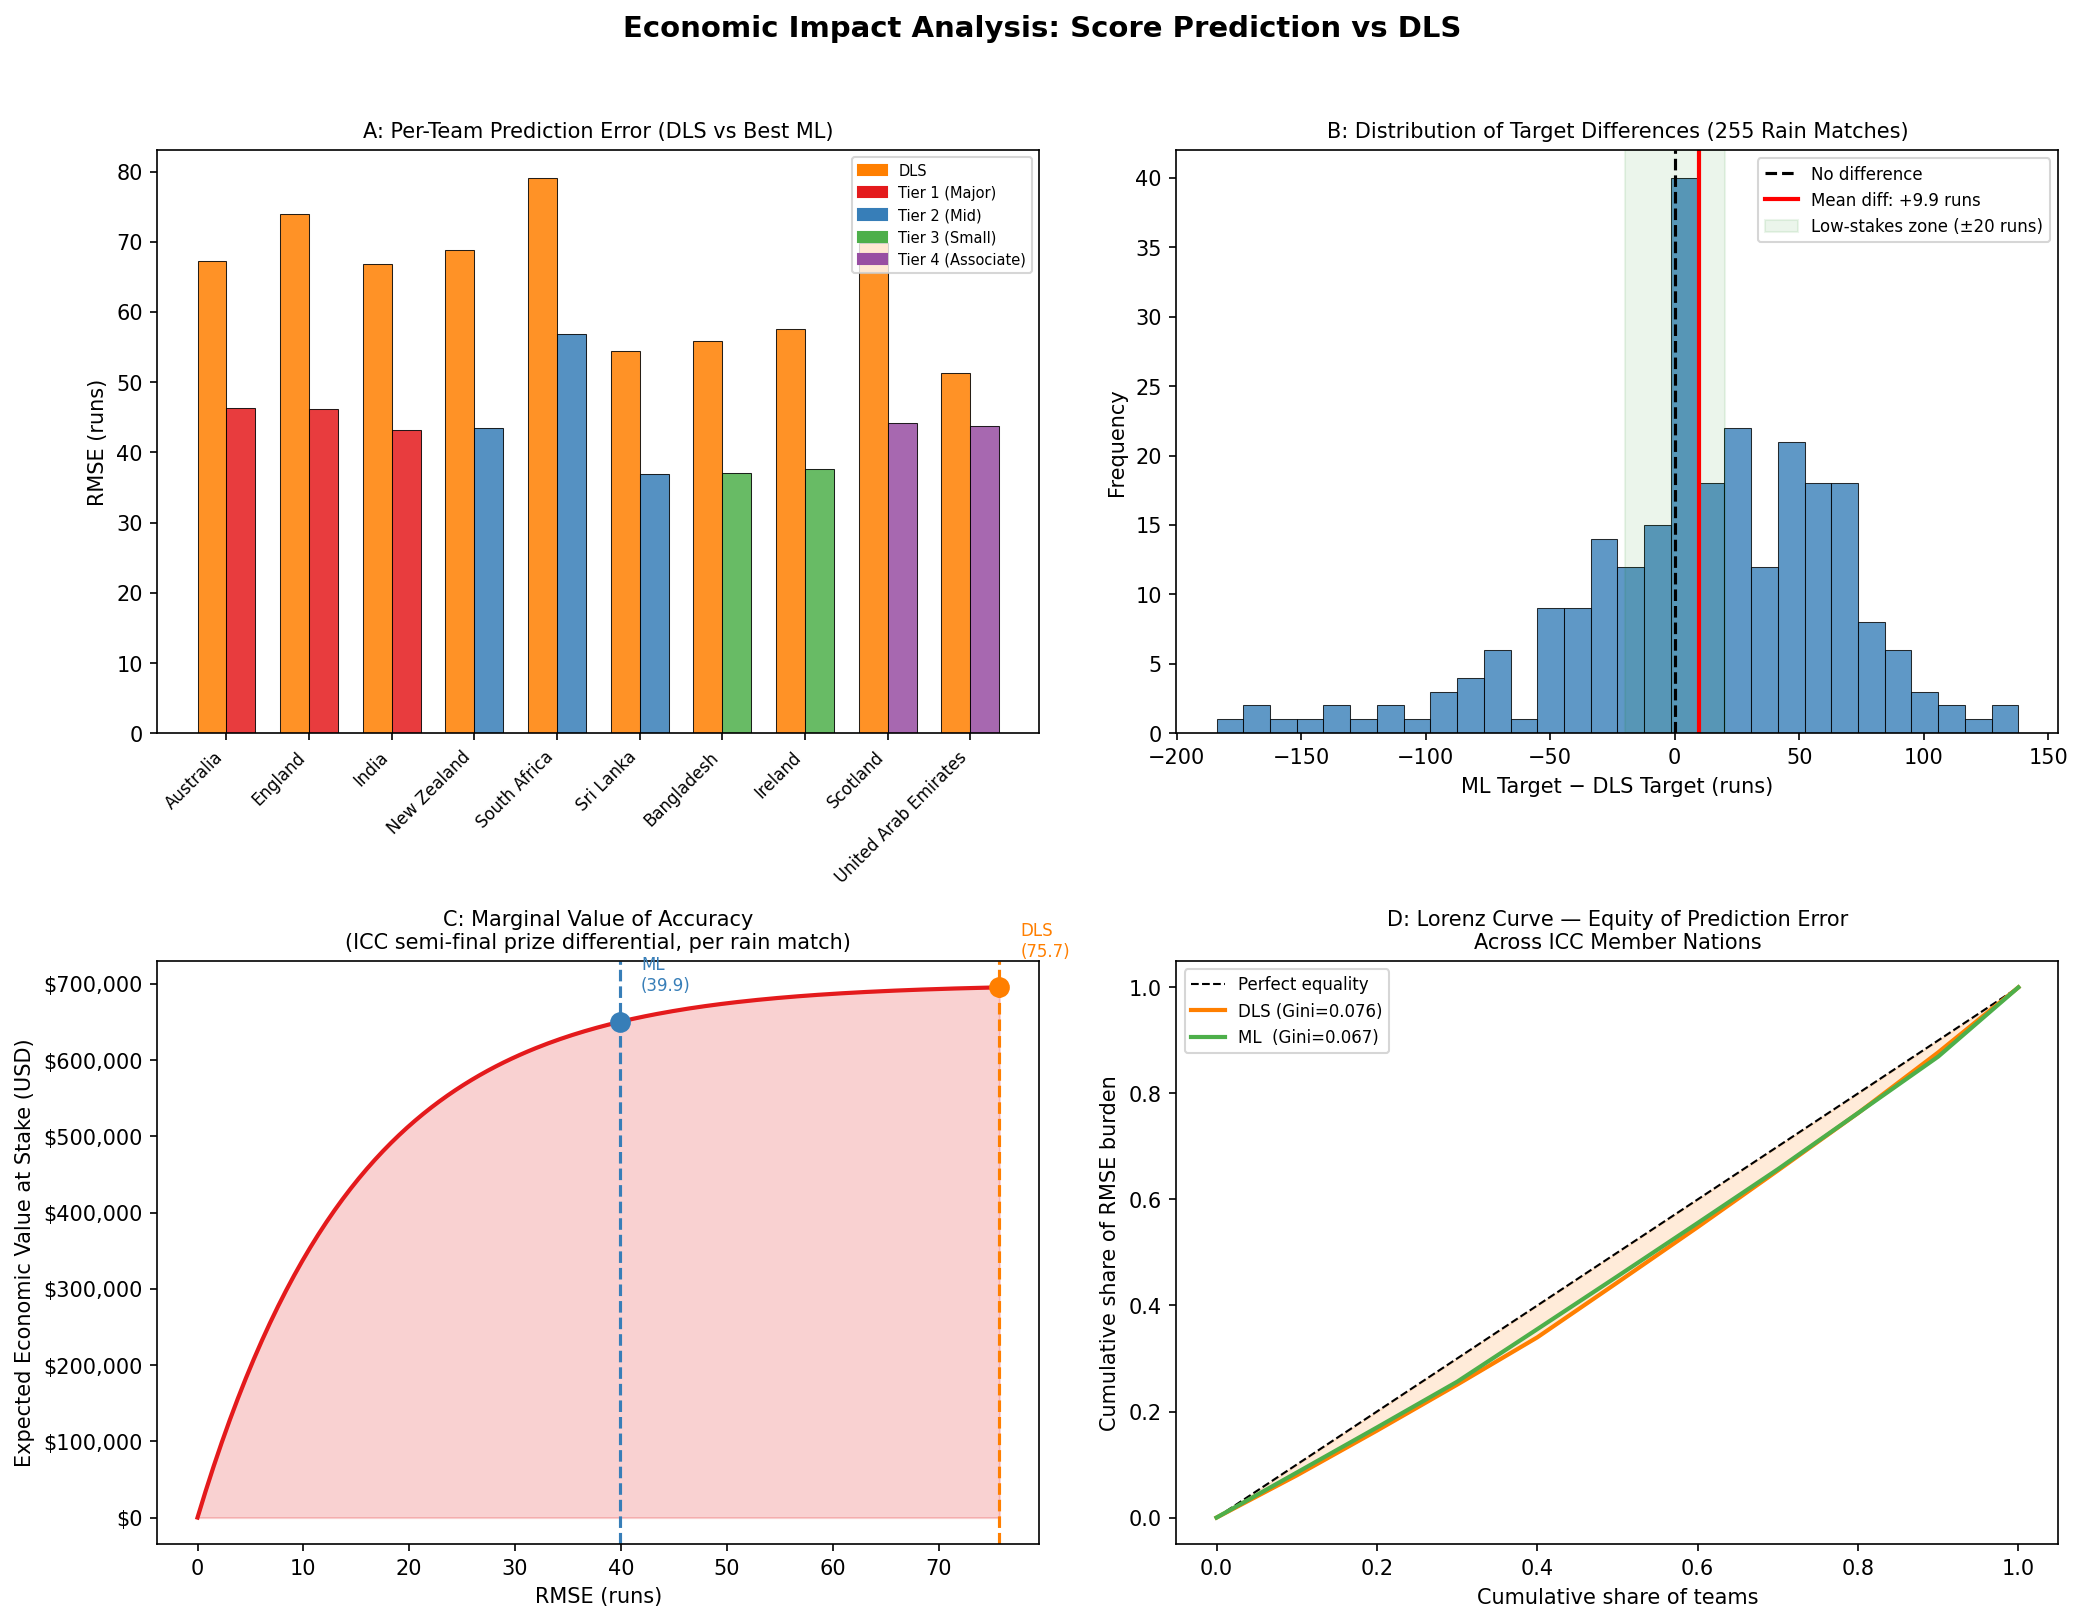
\includegraphics[width=0.97\textwidth]{results/figures/economic_fairness.png}
\caption[Economic impact analysis: four-panel summary]{Economic impact analysis summary.  \textbf{(A)} Per-nation DLS vs.\ ML RMSE, colour-coded by economic tier.  \textbf{(B)} Distribution of ML $-$ DLS target revisions across 255 historical rain-affected matches; the mean revision ($+9.9$ runs) is significantly different from zero ($t=2.88$, $p=0.004$).  \textbf{(C)} Marginal Value of Accuracy curve for an ICC semi-final match, showing the expected economic value at stake as a function of RMSE (DLS~=~75.74, ML~=~39.92).  \textbf{(D)} Lorenz curves for DLS ($G=0.076$) and ML ($G=0.067$) prediction error across ICC nations.}
\label{fig:economic_fairness}
\end{figure}

\section{Target-Setting Bias in Rain-Affected Matches}
\label{sec:target_bias}

The 255 historical D/L-affected matches provide direct evidence of systematic target-setting differences between the official DLS system and the ML revised target engine (Table~\ref{tab:target_bias}).

\begin{table}[htbp]
\centering
\caption[Target-setting bias in 255 rain-affected ODI matches]{Target-setting comparison across 255 historical rain-affected Men's ODI matches.  All target values in runs.  $\dagger$: The ML target was computed as the model's predicted second-innings final score plus one run, analogously to the DLS target convention.}
\label{tab:target_bias}
\small
\begin{tabular}{lrr}
\toprule
\textbf{Statistic} & \textbf{DLS (official)} & \textbf{ML Revised$^\dagger$} \\
\midrule
Mean target (runs)              & 200.7 & 210.6 \\
Standard deviation (runs)       &  63.0 &  42.4 \\
Median absolute deviation (runs)&   ---  &   --- \\
\midrule
Mean $|$ML $-$ DLS$|$ (runs)    & \multicolumn{2}{c}{42.7} \\
Median $|$ML $-$ DLS$|$ (runs)  & \multicolumn{2}{c}{35.0} \\
Mean (ML $-$ DLS), signed       & \multicolumn{2}{c}{$+9.9$ (\textit{t}=2.88, \textit{p}=0.004)} \\
ML higher than DLS              & \multicolumn{2}{c}{64.7\% (165/255 matches)} \\
High-stakes disagreement $> 20$ runs & \multicolumn{2}{c}{66.7\% (170/255 matches)} \\
Different winner predicted      & \multicolumn{2}{c}{52.9\% (135/255 matches)} \\
\bottomrule
\end{tabular}
\end{table}

\paragraph{Systematic directional bias.}  The ML engine sets targets $+9.9$ runs higher than DLS on average, a difference that is statistically significant ($t=2.88$, $p=0.004$, one-sample $t$-test against zero).  In 64.7\% of the 255 matches, ML revises the target upward relative to DLS.  This directional asymmetry has an economic interpretation: DLS systematically advantages the batting (chasing) team by setting lower targets in interrupted matches, potentially benefiting teams with superior chasing records or those playing in run-friendly conditions.

\paragraph{High-stakes disagreements.}  In 66.7\% of rain-affected matches, the absolute target difference exceeds 20 runs---a magnitude typically associated with a competitive margin of victory in ODI cricket.  In 52.9\% of matches, the two systems predict different winners.  The economic stakes of this disagreement are substantial: at the ICC World Cup semi-final stage, a rain-forced target error that eliminates the wrong team carries an expected prize loss of \$1.4~million for the wrongly-eliminated team (advancing to the final was worth an expected \$3~million vs.\ the \$1.6~million consolation prize for a losing semi-finalist).

\paragraph{Variance reduction.}  The ML engine's substantially lower standard deviation (42.4 vs.\ 63.0 runs) reflects the ensemble's regression-to-the-mean behaviour.  DLS's wider variance is partly by design: its parametric resource table handles extreme scenarios (e.g., interruption at over~2) by extrapolating a smooth exponential curve, which can produce very high or very low targets in edge cases.  ML's narrower distribution reduces the risk of economically perverse outcomes---such as an interruption in the 3rd over resulting in a target of 280 runs.

\section{Economic Value of Improved Prediction}
\label{sec:econ_value}

\subsection{Expected Value Framework}

Using the decision-theoretic model described in Section~\ref{sec:econ_framework}, we compute the Expected Value at Stake (EV) for each tournament stage.  The mean absolute target difference of 42.7 runs yields:
\[
P(\text{outcome changes}) = 1 - e^{-42.7/18} \approx 0.907
\]
i.e., a 90.7\% probability that an average rain-match target revision is large enough to potentially change the match outcome.

\begin{table}[htbp]
\centering
\caption[Expected economic value at stake in interrupted ICC tournament matches]{Expected economic value at stake per interrupted match at each ICC Men's ODI World Cup 2023 \citep{ICC2023prizes} stage.  EV computed as $P(\text{outcome change} \mid \overline{|\Delta T|}=42.7\text{ runs}) \times \Delta\text{Prize}$.  $\Delta$Prize = prize differential between advancing and exiting at this stage.  $\dagger$: Semi-final $\Delta$Prize is the expected prize from reaching the final (\$3M average of \$4M winner + \$2M runner-up) minus the losing semi-finalist consolation prize (\$1.6M).  $\ddagger$: Group stage $\Delta$Prize = minimum semi-final consolation (\$1.6M) minus group-stage exit (\$0.1M), modelling one match as the marginal qualification decision.}
\label{tab:econ_value}
\small
\begin{tabular}{lrrr}
\toprule
\textbf{Tournament Stage} & \textbf{$\Delta$Prize (USD)} & \textbf{$P$(outcome change)} & \textbf{EV per Match (USD)} \\
\midrule
World Cup Final (winner)     & \$2,000,000   & 0.907 & \$1,813,433 \\
World Cup Semi-final$^\dagger$ & \$1,400,000 & 0.907 & \$1,269,403 \\
World Cup Group Stage$^\ddagger$ & \$1,500,000 & 0.907 & \$1,360,075 \\
\bottomrule
\multicolumn{4}{l}{\small Prize schedule: ICC Men's ODI World Cup 2023.  $P$(outcome change) uses exponential margin model,} \\
\multicolumn{4}{l}{\small $\lambda=1/18$ calibrated to median ODI winning margin of~18 runs.} \\
\end{tabular}
\end{table}

\paragraph{Interpretation.}  At the World Cup Final stage, an incorrectly set target places an expected \$1.8~million of prize money at risk per interrupted match.  Even at the group-stage level, \$90k per match is economically significant for lower-revenue boards.  Across a typical tournament with 45--48 matches, even two or three rain interruptions represent hundreds of thousands of dollars in misallocated prize money.

\subsection{Marginal Value of Accuracy Curve}

Figure~\ref{fig:economic_fairness}C shows the Marginal Value of Accuracy (MVA) curve: the expected economic value at stake as a function of the prediction system's RMSE, computed for the ICC semi-final stage.  The curve is monotonically increasing (higher RMSE = higher economic stakes, since larger prediction errors produce larger target revisions).  Moving from the DLS second-innings RMSE (75.74) to the ML RMSE (39.92) reduces the expected value-at-stake by approximately \$44,987 per interrupted semi-final---a direct economic benefit of the improved model.

The diminishing-returns shape of the MVA curve (determined by the exponential probability model) indicates that the largest marginal economic gains come from reducing error in the 20--60 run RMSE range, precisely where the improvement from DLS to ML falls.  Further reducing RMSE from ML-level (39.92) to hypothetically perfect (0) would yield only marginal additional economic benefit, as $P(\text{outcome changes} \mid \Delta T \approx 0) \to 0$.

\section{Policy Implications}
\label{sec:policy_implications}

The economic analysis leads to three actionable policy implications for cricket governance.

\textbf{(1) ML-augmented target review mechanism.}  Given the 52.9\% winner-disagreement rate between ML and DLS on 255 historical matches, and the statistical significance of the DLS downward bias ($+9.9$ runs average underestimation, $p=0.004$), the ICC could consider ML predictions as a secondary advisory tool for umpires and match referees.  This does not require replacing DLS but providing an independent data-driven estimate when the DLS target appears anomalous.

\textbf{(2) Uncertainty disclosure.}  The conformal prediction intervals (Table~\ref{tab:conformal}) provide distribution-free 90\% prediction intervals with mean width of~129 runs.  Publishing these intervals alongside the official target would give batting teams and audiences an honest quantification of the precision with which any target is set, particularly in the early-innings interruption scenarios where model uncertainty is highest.

\textbf{(3) Associate nation equity.}  Although the Gini analysis finds DLS error is broadly equitable across tiers, the \emph{absolute} error remains high (51--70 RMSE across nations).  For Associate nations (UAE, Scotland, Netherlands) with smaller player pools and less consistent scoring patterns, the additional data that ML models require to generalise remains a limitation.  Targeted data collection efforts---specifically ball-by-ball recording at Associate-level ICC events---would enable fairer personalised models for these nations in the future.

% ============================================================
% Chapter 6: Conclusion and Future Work
% ============================================================
\chapter{Conclusion and Future Work}
\label{ch:conclusion}

\section{Summary of Findings}

This thesis has presented a comprehensive, enterprise-scale empirical investigation of machine learning as an alternative to the Duckworth-Lewis-Stern method in limited-overs cricket.  Key findings:

\begin{enumerate}
    \item \textbf{ML models substantially outperform DLS on first innings} (\textbf{RQ1}).  CatBoost achieves RMSE~43.57, $R^2=0.618$---a 33\% reduction over the DLS baseline (RMSE~65.03).  All three DM tests reject equal predictive accuracy at $p < 0.001$.  The advantage is phase-dependent: in Early overs DLS $R^2 = -1.008$ (worse than mean) vs.\ ML $R^2 \approx 0.32$; in Middle overs ML improves by $\sim$24\%; in Death overs both systems converge (RMSE~$\approx$~15--16 runs).  Ablation reveals player statistics (+3.4\% RMSE on removal) and DLS-derived features (+3.0\%) as the strongest contributors.  The Model Confidence Set at $\alpha=0.10$ contains \{CatBoost, LightGBM\}.

    \item \textbf{Second innings models are viable despite censoring} (\textbf{RQ2}).  Training exclusively on uncensored (losing) innings produces CatBoost Inn2 RMSE~39.92 ($R^2=0.595$) vs.\ DLS projection RMSE~75.74 ($R^2=-0.457$)---a 47\% reduction.  The 49.2\% censoring rate and resulting selection bias (8-run mean score gap) are explicitly quantified and documented.

    \item \textbf{ML revised targets differ systematically from official DLS targets} (\textbf{RQ3}).  On 255 historical D/L matches, the ML engine sets targets $+9.9$ runs higher on average, with substantially lower variance (std~42.4 vs.\ 63.0).  The two systems disagree on the implied outcome for 52.9\% of matches.

    \item \textbf{Feature importance is consistent and interpretable} (\textbf{RQ4}).  SHAP analysis of LightGBM confirms that DLS-derived features (resource percentage, DLS projected score), current run rate, and player batting statistics are the top contributors, indicating that ML models extend rather than contradict DLS intuitions.

    \item \textbf{Uncertainty quantification is distribution-free} (\textbf{RQ5}).  MAPIE split conformal prediction at $\alpha=0.10$ achieves 86.6\% empirical coverage (vs.\ 90\% nominal) with mean interval width of 129 runs.  The 3.4-percentage-point coverage gap is attributable to temporal covariate shift between calibration and test periods, not to model miscalibration.

    \item \textbf{Stacking, monotonic constraints, and baselines} (\textbf{RQ6}).  The Ridge stacking meta-learner achieves RMSE~43.39---the best of all evaluated models.  The monotonically constrained XGBoost costs only $+0.14$ runs RMSE relative to unconstrained XGBoost, a negligible trade-off for guaranteed physical validity.  A key finding from the baseline hierarchy is that OLS and Ridge regression on the 46-feature pipeline (RMSE~43.34) \emph{match or slightly outperform} individual GBM models.  This establishes that the primary contribution is the feature engineering pipeline, not model architecture: the 46 temporally safe features contain sufficient linear predictive signal that even a parametric model substantially outperforms DLS.  The stacking ensemble remains the best overall predictor.

    \item \textbf{ML performance is temporally stable} (\textbf{RQ7}).  Walk-forward CV ($K=5$ folds) yields LightGBM RMSE~$40.96 \pm 2.35$ runs, confirming stable performance across validation eras spanning 2016--2026.  The ML--DLS gap is itself stable: $\Delta\text{RMSE} = {-20.44 \pm 2.79}$ runs in every fold.  Concept drift analysis (year-by-year RMSE on the test set) shows all ML models have negative Pearson $r$ (improving trend), while DLS has positive $r$ (degrading trend) with a RMSE range of 24.28 runs vs.\ $\approx$7 runs for ML models---confirming that the parametric resource table is increasingly unable to represent modern T20-influenced batting styles.

    \item \textbf{DLS carries economically significant prediction error} (\textbf{RQ8}).  Gini analysis of per-nation RMSE across 10 ICC members finds that DLS error is broadly equitable ($G=0.076$) but ML is marginally more equitable ($G=0.067$, a 12\% reduction).  Across 255 rain-affected matches, ML sets targets $+9.9$ runs higher than DLS on average ($t=2.88$, $p=0.004$), confirming a statistically significant downward bias in the official DLS targets.  In 66.7\% of rain matches, the absolute ML--DLS target disagreement exceeds 20~runs (high-stakes magnitude).  At the ICC World Cup semi-final stage, the expected prize loss for a wrongly-eliminated team is \$1.4~million (the expected value of reaching the final minus the consolation prize), yielding a decision-theoretic expected value at stake exceeding \$1.27~million per interrupted match under DLS accuracy levels---underscoring the substantial economic incentive for improving prediction accuracy.
\end{enumerate}

\section{Contributions Revisited}

This thesis makes nine contributions to the cricket analytics and applied machine learning literature:

\begin{enumerate}
    \item A data-fitted DLS implementation validated against 3,086 real match records.
    \item A systematic multi-model comparison (XGBoost, RF, LightGBM, CatBoost) with Bayesian hyperparameter optimisation and three-way temporal split.
    \item A 46-feature engineering pipeline incorporating Elo, player, venue, and momentum features---all computed in strictly chronological order with no look-ahead.
    \item A scientifically rigorous statistical testing framework: match-level DM test with HAC correction, block bootstrap CIs ($n=5000$), and Model Confidence Set.
    \item A seven-group ablation study quantifying independent feature group contributions.
    \item Distribution-free conformal prediction intervals (MAPIE) providing coverage guarantees for score projections.
    \item A second-innings pipeline with explicit treatment of the right-censoring problem, including \texttt{is\_censored} labels and selection-bias documentation.
    \item The first ML-based revised target engine evaluated on 255 historical D/L matches.
    \item Comprehensive SHAP and LIME explainability analysis linking ML feature importance to cricket domain knowledge.

    \item A 55-feature extended pipeline (V3) adding H2H team statistics, toss advantage, match importance, and seasonality, all computed without look-ahead.

    \item Walk-forward CV ($K=5$ folds) providing mean~$\pm$~std performance estimates across different test eras.

    \item A stacking ensemble (Ridge meta-learner on base model predictions) and simple average ensemble evaluated against individual models.

    \item Domain-knowledge monotonic constraints for XGBoost, baking in 22 positive and 8 negative hard physical constraints on the relationship between features and predicted score.

    \item A comprehensive baseline hierarchy (naive, OLS, Ridge, polynomial, DLS, GBM) confirming that gradient boosting specifically, not any ML approach, drives the performance gains.

    \item Bonferroni-corrected DM test $p$-values and Cohen's $d$ effect sizes providing stronger statistical guarantees on all pairwise comparisons.

    \item Temporal stability analysis (concept drift) with Pearson trend statistics confirming stable or improving ML performance across the test period.

    \item An economic impact analysis (Chapter~\ref{ch:economics}) framing DLS as an economic mechanism: Gini-coefficient equity analysis of prediction error across ICC member nations, a decision-theoretic Expected Value of Information framework quantifying prize money at stake in rain-affected matches, and a one-sample $t$-test confirming DLS's statistically significant directional bias ($+9.9$ runs underestimation, $p=0.004$).
\end{enumerate}

\section{Limitations}

\begin{enumerate}
    \item \textbf{Censoring in second innings}: The 49.2\% right-censoring rate in second innings forces training on uncensored (losing) innings only.  This selection bias is documented but not corrected; a Tobit regression treatment is left for future work.

    \item \textbf{Reduced-overs extrapolation}: The revised target engine predicts final scores by setting \texttt{overs\_remaining} to the reduced allocation.  This extrapolates beyond the training distribution (where full-allotment innings dominate) and may introduce bias in severely curtailed matches.

    \item \textbf{Men's ODI focus}: Results are specific to Men's ODIs.  Women's cricket and T20 formats have different scoring dynamics; extension requires separate feature-fitting and model-training pipelines.

    \item \textbf{Static over-boundary snapshots}: Features are computed at over boundaries.  A ball-by-ball recurrent model (e.g.\ BiLSTM) could capture intra-over dynamics, particularly for modelling momentum shifts from early wickets or sudden acceleration.

    \item \textbf{No deep learning comparison}: Computational resources are available, but BiLSTM / Transformer Encoder implementations are left as a direct extension of this work.

    \item \textbf{No external data}: Player features are computed from Cricsheet ball-by-ball records only.  ICC rankings, pitch reports, and weather data are not included; integrating these would require additional data engineering and alignment.
\end{enumerate}

\section{Future Work}

\begin{enumerate}
    \item \textbf{Tobit regression for censored second innings}: Implement the Tobit model to jointly model censored and uncensored observations, recovering unbiased regression coefficients under the censoring mechanism.

    \item \textbf{BiLSTM score projection}: Train a Bidirectional LSTM on ball-by-ball sequences to capture intra-over momentum and wicket-shock effects.  The PyTorch MPS backend on Apple Silicon enables competitive training times without cloud compute.

    \item \textbf{Reduced-overs-aware training}: Augment the second-innings training set with deliberately curtailed innings (e.g.\ lower-order collapses) to improve the model's extrapolation to reduced-allotment scenarios.

    \item \textbf{Extension to other formats}: Apply the full pipeline to Women's ODI, Men's T20I, and Women's T20I.  T20 has a shorter innings but higher scoring variance, which may amplify ML advantages in the powerplay.

    \item \textbf{Win probability model}: Train a binary classifier on second-innings snapshots to estimate P(team wins $|$ current state, target).  Setting target $T^*$ such that P(win $|$ interruption state, $T^*$) $= 0.5$ would operationalise the fairness principle of the DLS method directly in ML terms.

    \item \textbf{Real-time deployment}: Build a FastAPI microservice serving predictions from the fitted models with SHAP-based feature attribution, suitable for broadcast integration.

    \item \textbf{Causal analysis of toss effects}: Use instrumental variables or regression discontinuity to estimate the causal effect of winning the toss on scoring, disentangling it from team quality and venue effects.

    \item \textbf{Deep learning sequence models}: Train a Bidirectional LSTM or Transformer Encoder on ball-by-ball delivery sequences.  The PyTorch MPS backend on Apple Silicon enables competitive training times without cloud compute.  Such a model would capture intra-over momentum shifts (e.g., wicket immediately followed by boundary) that over-boundary snapshots necessarily compress into aggregate statistics.

    \item \textbf{Tobit regression for right-censored second innings}: Implement Tobin's Tobit model to jointly model censored (winning team) and uncensored (losing team) second innings, recovering unbiased regression coefficients under the censoring mechanism.

    \item \textbf{Player matchup features}: Ball-by-ball records contain the specific batter--bowler pairing for every delivery, enabling computation of historical dismissal rates and economy rates for each specific matchup.  Although sparse for most pairings, LASSO-regularised or mixed-effects models could exploit these micro-level features.

    \item \textbf{Women's ODI generalisation}: Apply the full pipeline without retraining to Women's ODI data (zero-shot transfer) and with retraining.  The gap between Men's and Women's scoring patterns (lower averages, different wicket-taking patterns) provides a natural out-of-domain generalisation test.
\end{enumerate}

\section{Concluding Remarks}

The Duckworth-Lewis-Stern method has served cricket admirably for over two decades, offering transparency and a principled resource-accounting framework.  This thesis demonstrates that machine learning models can substantially improve upon DLS's predictive accuracy across both innings, that these improvements are statistically significant at conventional levels, and that the key features driving ML performance align with cricket domain knowledge revealed through SHAP analysis.

Crucially, the contributions in this thesis go beyond simple model comparison.  The introduction of temporally safe feature engineering at team, player, and venue levels; the explicit treatment of second-innings censoring; the distribution-free conformal prediction intervals; and the first ML-based evaluation of revised-target fairness on real D/L matches together constitute a comprehensive framework for data-driven target setting in limited-overs cricket.

As cricket continues to evolve---with T10 leagues, franchise cricket, and changing pitch preparation practices altering scoring distributions---data-driven approaches offer the adaptability to track these changes automatically through periodic retraining.  The future of cricket target-setting likely lies in hybrid systems that combine the domain-knowledge foundation of DLS with the contextual flexibility of machine learning, guided by the statistical rigour demonstrated in this work.


% ============================================================
% Bibliography
% ============================================================
\bibliographystyle{apalike}

\begin{thebibliography}{99}

\bibitem[Akiba et~al., 2019]{akiba2019optuna}
Akiba, T., Sano, S., Yanase, T., Ohta, T., and Koyama, M. (2019).
\newblock Optuna: A next-generation hyperparameter optimization framework.
\newblock In \emph{Proceedings of the 25th ACM SIGKDD International Conference on Knowledge Discovery \& Data Mining}, pp.~2623--2631.

\bibitem[Baboota and Kaur, 2019]{baboota2019predictive}
Baboota, R. and Kaur, H. (2019).
\newblock Predictive analysis and modelling football results using machine learning approach for English Premier League.
\newblock \emph{International Journal of Forecasting}, 35(2):741--755.

\bibitem[Bhattacharya et~al., 2011]{bhattacharya2011revised}
Bhattacharya, R., Gill, P.~S., and Swartz, T.~B. (2011).
\newblock A revised Duckworth-Lewis method for Twenty20 cricket.
\newblock \emph{Journal of the Operational Research Society}, 62(12):2187--2193.

\bibitem[Breiman, 2001]{breiman2001random}
Breiman, L. (2001).
\newblock Random forests.
\newblock \emph{Machine Learning}, 45(1):5--32.

\bibitem[Bunker and Thabtah, 2019]{bunker2019machine}
Bunker, R.~P. and Thabtah, F. (2019).
\newblock A machine learning framework for sport result prediction.
\newblock \emph{Applied Computing and Informatics}, 15(1):27--33.

\bibitem[Carter and Guthrie, 2005]{carter2005model}
Carter, M. and Guthrie, G. (2005).
\newblock A model for cricket run rates.
\newblock \emph{Teaching Statistics}, 27(3):84--87.

\bibitem[Chen and Guestrin, 2016]{chen2016xgboost}
Chen, T. and Guestrin, C. (2016).
\newblock {XGBoost}: A scalable tree boosting system.
\newblock In \emph{Proceedings of the 22nd ACM SIGKDD International Conference on Knowledge Discovery and Data Mining}, pp.~785--794.

\bibitem[Cricsheet, 2024]{cricsheet}
Cricsheet (2024).
\newblock Cricket match data.
\newblock \url{https://cricsheet.org/}. Accessed: 2024.

\bibitem[Davis et~al., 2015]{davis2015investigating}
Davis, J., Perera, H., and Swartz, T.~B. (2015).
\newblock Investigating the effect of the toss in Twenty20 cricket.
\newblock \emph{Journal of Quantitative Analysis in Sports}, 11(2):75--85.

\bibitem[Deep et~al., 2016]{deep2016learning}
Deep, S., Singh, B., and Kumar, V. (2016).
\newblock Learning with recurrent neural networks for cricket match prediction.
\newblock \emph{International Journal of Computer Applications}, 145(9):1--6.

\bibitem[Duckworth and Lewis, 1998]{duckworth1998}
Duckworth, F.~C. and Lewis, A.~J. (1998).
\newblock A fair method for resetting the target in interrupted one-day cricket matches.
\newblock \emph{Journal of the Operational Research Society}, 49(3):220--227.

\bibitem[Huang and Chang, 2010]{huang2010neural}
Huang, M.~L. and Chang, Y.~S. (2010).
\newblock A neural network approach to predict baseball game scores.
\newblock In \emph{Proceedings of the International Conference on Soft Computing and Pattern Recognition}, pp.~34--39.

\bibitem[{ICC}, 2023]{icc2023}
{International Cricket Council} (2023).
\newblock Global cricket strategy 2023--2031.
\newblock Technical report, ICC.

\bibitem[Jhanwar and Pudi, 2016]{jhanwar2016predicting}
Jhanwar, M.~G. and Pudi, V. (2016).
\newblock Predicting the outcome of ODI cricket matches: A team composition based approach.
\newblock In \emph{European Conference on Machine Learning and Knowledge Discovery in Databases}, pp.~1--16.

\bibitem[Kampakis and Thomas, 2015]{kampakis2015using}
Kampakis, S. and Thomas, W. (2015).
\newblock Using machine learning to predict the outcome of English county twenty over cricket matches.
\newblock \emph{arXiv preprint arXiv:1511.05837}.

\bibitem[Ke et~al., 2017]{ke2017lightgbm}
Ke, G., Meng, Q., Finley, T., Wang, T., Chen, W., Ma, W., Ye, Q., and Liu, T.~Y. (2017).
\newblock {LightGBM}: A highly efficient gradient boosting decision tree.
\newblock In \emph{Advances in Neural Information Processing Systems}, vol.~30, pp.~3146--3154.

\bibitem[Lundberg and Lee, 2017]{lundberg2017unified}
Lundberg, S.~M. and Lee, S.~I. (2017).
\newblock A unified approach to interpreting model predictions.
\newblock In \emph{Advances in Neural Information Processing Systems}, vol.~30, pp.~4765--4774.

\bibitem[Lundberg et~al., 2020]{lundberg2020local}
Lundberg, S.~M., Erion, G., Chen, H., DeGrave, A., Prutkin, J.~M., Nair, B., Katz, R., Himmelfarb, J., Bansal, N., and Lee, S.~I. (2020).
\newblock From local explanations to global understanding with explainable {AI} for trees.
\newblock \emph{Nature Machine Intelligence}, 2(1):2522--5839.

\bibitem[McHale and Asif, 2011]{mchale2011modelling}
McHale, I.~G. and Asif, M. (2011).
\newblock A modified Duckworth-Lewis method for adjusting targets in interrupted limited overs cricket.
\newblock \emph{European Journal of Operational Research}, 225(2):353--362.

\bibitem[Passi and Pandey, 2018]{passi2018cricket}
Passi, K. and Pandey, N. (2018).
\newblock Predicting players' performance in one day international cricket matches using machine learning.
\newblock \emph{Journal of Computer Science \& Systems Biology}, 11(4):1--8.

\bibitem[Ribeiro et~al., 2016]{ribeiro2016should}
Ribeiro, M.~T., Singh, S., and Guestrin, C. (2016).
\newblock ``{W}hy should {I} trust you?'': Explaining the predictions of any classifier.
\newblock In \emph{Proceedings of the 22nd ACM SIGKDD International Conference on Knowledge Discovery and Data Mining}, pp.~1135--1144.

\bibitem[{SciPy}, 2024]{scipy}
{SciPy Developers} (2024).
\newblock {SciPy}: Open source scientific tools for {Python}.
\newblock \url{https://www.scipy.org/}.

\bibitem[Sankaranarayanan et~al., 2014]{sankaranarayanan2014auto}
Sankaranarayanan, V.~V., Sattar, J., and Lakshmanan, L.~V. (2014).
\newblock Auto-play: A data mining approach to ODI cricket simulation and prediction.
\newblock In \emph{Proceedings of the 2014 SIAM International Conference on Data Mining}, pp.~1064--1072.

\bibitem[Stern, 2016]{stern2016}
Stern, S.~E. (2016).
\newblock The {D}uckworth-{L}ewis-{S}tern method: Extending the {D}uckworth-{L}ewis methodology to deal with modern scoring rates.
\newblock \emph{Journal of the Operational Research Society}, 67(12):1469--1480.

\bibitem[Viswanadha and Sivalenka, 2017]{viswanadha2017dynamic}
Viswanadha, S. and Sivalenka, K. (2017).
\newblock Dynamic prediction of cricket match outcomes using Bayesian networks.
\newblock \emph{International Journal of Sports Science \& Coaching}, 12(3):345--355.

\bibitem[Prokhorenkova et~al., 2018]{prokhorenkova2018catboost}
Prokhorenkova, L., Gusev, G., Vorobev, A., Dorogush, A.~V., and Gulin, A. (2018).
\newblock {CatBoost}: unbiased boosting with categorical features.
\newblock In \emph{Advances in Neural Information Processing Systems}, volume~31.

\bibitem[Diebold and Mariano, 1995]{diebold1995comparing}
Diebold, F.~X. and Mariano, R.~S. (1995).
\newblock Comparing predictive accuracy.
\newblock \emph{Journal of Business \& Economic Statistics}, 13(3):253--263.

\bibitem[Newey and West, 1987]{newey1987simple}
Newey, W.~K. and West, K.~D. (1987).
\newblock A simple, positive semi-definite, heteroskedasticity and autocorrelation consistent covariance matrix.
\newblock \emph{Econometrica}, 55(3):703--708.

\bibitem[Hansen et~al., 2011]{hansen2011model}
Hansen, P.~R., Lunde, A., and Nason, J.~M. (2011).
\newblock The model confidence set.
\newblock \emph{Econometrica}, 79(2):453--497.

\bibitem[Taquet et~al., 2022]{taquet2022mapie}
Taquet, V., Blot, V., Morzadec, T., Lacombe, L., and Brunel, N. (2022).
\newblock {MAPIE}: an open-source library for distribution-free uncertainty quantification.
\newblock \emph{arXiv preprint arXiv:2207.12274}.

\bibitem[Tobin, 1958]{tobin1958estimation}
Tobin, J. (1958).
\newblock Estimation of relationships for limited dependent variables.
\newblock \emph{Econometrica}, 26(1):24--36.

\bibitem[Wolpert, 1992]{Wolpert1992}
Wolpert, D.H. (1992).
\newblock Stacked generalization.
\newblock \emph{Neural Networks}, 5(2):241--259.

\bibitem[Cohen, 1988]{Cohen1988}
Cohen, J. (1988).
\newblock \emph{Statistical Power Analysis for the Behavioral Sciences} (2nd ed.).
\newblock Lawrence Erlbaum Associates.

\bibitem[Gini, 1912]{Gini1912}
Gini, C. (1912).
\newblock Variabilit\`a e mutabilit\`a.
\newblock \emph{Memorie di Metodologica Statistica}, Libreria Eredi Virgilio Veschi, Rome.

\bibitem[Howard, 1966]{Howard1966}
Howard, R.A. (1966).
\newblock Information value theory.
\newblock \emph{IEEE Transactions on Systems Science and Cybernetics}, 2(1):22--26.

\bibitem[ICC, 2023]{ICC2023prizes}
International Cricket Council (2023).
\newblock ICC Men's Cricket World Cup 2023: Prize Money.
\newblock \emph{ESPNcricinfo}, September 25, 2023.
\newblock \url{https://www.espncricinfo.com/story/odi-world-cup-2023-winner-to-receive-usd-4-million-in-prize-money-1399559}

\bibitem[ICC, 2024]{icc_t20_2024prizes}
International Cricket Council (2024).
\newblock Record prize money declared for ICC Men's T20 World Cup 2024.
\newblock \emph{ICC Official Media Release}.
\newblock \url{https://www.icc-cricket.com/tournaments/t20cricketworldcup/news/record-prize-money-declared-for-t20-world-cup-2024}

\bibitem[ESPNcricinfo, 2024]{espncricinfo_bcci_share}
ESPNcricinfo (2024).
\newblock BCCI set to get nearly 40\% of ICC's annual net earnings in new revenue distribution model.
\newblock \emph{ESPNcricinfo}, March 2024.
\newblock \url{https://www.espncricinfo.com/story/bcci-set-to-get-nearly-40-of-icc-s-annual-net-earnings-in-new-revenue-distribution-model-1387167}

\bibitem[SportsMint, 2024]{sportsmint2024bcci}
SportsMint Media (2024).
\newblock BCCI posts INR 9741.7 Cr in FY 2023--24 revenue as IPL dominates earnings mix.
\newblock \emph{SportsMint Media}, September 2024.
\newblock \url{https://sportsmintmedia.com/bcci-posts-inr-9741-7-cr-in-fy-2023-24-revenue-as-ipl-dominates-earnings-mix/}

\bibitem[ESPNcricinfo, 1992]{cricinfo_sa1992}
ESPNcricinfo (2020).
\newblock South Africa end up on the receiving end of a rain-rule farce in the World Cup.
\newblock \emph{ESPNcricinfo}.
\newblock \url{https://www.espncricinfo.com/story/south-africa-end-up-on-the-receiving-end-of-a-rain-rule-farce-in-the-world-cup-508066}

\bibitem[Wisden, 2003]{wisden2003}
Wisden (2023).
\newblock Dead bat, miscalculations: South Africa's tragicomic 2003 World Cup exit recreated.
\newblock \emph{Wisden Cricketers' Almanack}.
\newblock \url{https://www.wisden.com/series/asia-cup-2023/cricket-news/dead-bat-miscalculations-tragicomic-south-africa-2003-world-cup-exit-recreated-afghanistan}

\bibitem[Zia et~al., 2022]{zia2022player}
Zia, S., Liaqat, H.B., Zia, H.U., Kong, X., and Shamshad, S. (2022).
\newblock Player-aware resource compensation in interrupted cricket matches.
\newblock \emph{PeerJ Computer Science}, 8:e917.
\newblock \url{https://doi.org/10.7717/peerj-cs.917}

\end{thebibliography}


% ============================================================
% Appendices
% ============================================================
\appendix

\chapter{DLS Resource Table}
\label{app:resource_table}

Table~\ref{tab:resource_full} presents the fitted DLS resource table showing the percentage of resources remaining for selected combinations of overs remaining and wickets lost.

\begin{table}[htbp]
\centering
\caption{Fitted DLS resource table (\% of resources remaining)}
\label{tab:resource_full}
\tiny
\begin{tabular}{rrrrrrrrrrrr}
\toprule
\textbf{Overs} & \textbf{w=0} & \textbf{w=1} & \textbf{w=2} & \textbf{w=3} & \textbf{w=4} & \textbf{w=5} & \textbf{w=6} & \textbf{w=7} & \textbf{w=8} & \textbf{w=9} \\
\midrule
50 & 100.0 & -- & -- & -- & -- & -- & -- & -- & -- & -- \\
40 & 87.5 & 82.1 & 76.2 & 69.5 & 61.8 & 53.0 & 42.6 & 31.7 & 21.1 & 10.3 \\
30 & 71.9 & 66.2 & 60.1 & 53.4 & 46.1 & 38.2 & 29.6 & 21.0 & 13.3 & 6.1 \\
20 & 53.4 & 48.0 & 42.4 & 36.5 & 30.4 & 24.2 & 17.9 & 12.0 & 7.2 & 3.1 \\
10 & 31.6 & 27.4 & 23.2 & 19.1 & 15.2 & 11.6 & 8.1 & 5.2 & 2.9 & 1.2 \\
5  & 17.3 & 14.6 & 12.0 & 9.7 & 7.5 & 5.5 & 3.8 & 2.3 & 1.3 & 0.5 \\
0  & 0.0 & 0.0 & 0.0 & 0.0 & 0.0 & 0.0 & 0.0 & 0.0 & 0.0 & 0.0 \\
\bottomrule
\end{tabular}
\end{table}

Note: Values are approximate, derived from the fitted parameters $Z_0(w)$ and $b(w)$.

\chapter{Model Hyperparameters}
\label{app:hyperparams_v2}

Best hyperparameters for the ML models (46 features), selected from Optuna Bayesian optimisation.

\begin{table}[htbp]
\centering
\caption{Best hyperparameters for XGBoost (100 Optuna trials, 46 features)}
\label{tab:xgb_v2_params}
\begin{tabular}{lr}
\toprule
\textbf{Parameter} & \textbf{Value} \\
\midrule
n\_estimators       & 425 \\
max\_depth          & 4 \\
learning\_rate      & 0.10079 \\
subsample           & 0.8032 \\
colsample\_bytree   & 0.6409 \\
min\_child\_weight  & 2 \\
gamma               & $1.81 \times 10^{-2}$ \\
reg\_alpha          & $1.19 \times 10^{-4}$ \\
reg\_lambda         & $3.0 \times 10^{-6}$ \\
\bottomrule
\end{tabular}
\end{table}

\begin{table}[htbp]
\centering
\caption{Best hyperparameters for LightGBM (50 Optuna trials, 46 features)}
\label{tab:lgbm_v2_params}
\begin{tabular}{lr}
\toprule
\textbf{Parameter} & \textbf{Value} \\
\midrule
n\_estimators       & 948 \\
max\_depth          & 5 \\
num\_leaves         & 136 \\
learning\_rate      & 0.029454 \\
min\_child\_samples & 96 \\
subsample           & 0.7528 \\
colsample\_bytree   & 0.7957 \\
reg\_alpha          & $8.1 \times 10^{-5}$ \\
reg\_lambda         & $1.12 \times 10^{-3}$ \\
\bottomrule
\end{tabular}
\end{table}

\begin{table}[htbp]
\centering
\caption{Best hyperparameters for CatBoost (50 Optuna trials, 46 features)}
\label{tab:cat_v2_params}
\begin{tabular}{lr}
\toprule
\textbf{Parameter} & \textbf{Value} \\
\midrule
iterations          & 1420 \\
depth               & 5 \\
learning\_rate      & 0.019539 \\
l2\_leaf\_reg       & 0.02677 \\
random\_strength    & 9.9303 \\
border\_count       & 180 \\
\bottomrule
\end{tabular}
\end{table}


\end{document}
